\documentclass[]{spie}  % SPIE Proceedings format (US Letter)

\usepackage[]{graphicx}
\usepackage{amsmath,amssymb,amsfonts}
\usepackage{booktabs}
\usepackage{multirow}
\usepackage{url}
\usepackage{hyperref}

\hypersetup{
    colorlinks=true,
    linkcolor=blue,
    citecolor=blue,
    urlcolor=blue
}

% -------------------------------------------------------------------------
% TITLE AND AUTHOR INFORMATION
% NOTE: For single-blind submission (ADIP / SPIE standard), please insert 
% your real names, affiliations, and correspondence email below.
% If submitting as double-blind, keep "Anonymous Authors".
% -------------------------------------------------------------------------
\title{Calibrated Hybrid Geometry--Learning Monocular Vehicle Distance Estimation with Lightweight YOLO Detectors}

\author{Nguyen Quang Thang\supit{a}, Tran Quoc Trieu\supit{a}, Hoang Anh Tuan\supit{a}, and Cao Van Mai\supit{a}
\skiplinehalf
\supit{a}FPT University, Hanoi, Vietnam
}

\authorinfo{Further author information: (Send correspondence to Nguyen Quang Thang)\\
Nguyen Quang Thang: E-mail: nguyenthang060706@gmail.com\\
Tran Quoc Trieu: E-mail: tranquoctrieu382006@gmail.com\\
Hoang Anh Tuan: E-mail: tuanhoang101106@gmail.com\\
Cao Van Mai: E-mail: maicv2@fe.edu.vn}

\begin{document}
\maketitle

% -------------------------------------------------------------------------
% ABSTRACT
% -------------------------------------------------------------------------
\begin{abstract}
Estimating the distance of preceding vehicles using a single monocular camera is a vital task for advanced driver assistance systems (ADAS) and autonomous driving under stringent computational constraints. While deep learning models offer competitive precision, direct depth regression lacks physical explainability and operates without transparent error attribution to optical geometry or 2D detector bounding box localization. Conversely, pure pinhole geometry offers explicit physical grounding but suffers from systematic biases due to vehicle orientation, 3D center-to-surface offset, and boundary clipping. In this work, we present a calibrated hybrid monocular distance estimation framework integrating perspective geometry with learned residual correction and conformalized quantile regression (CQR). Three pinhole cues (width, height, and ground-plane constraint) are fused via empirical covariance-weighted log-space pooling to establish a physically grounded baseline. A lightweight gradient-boosted residual model compensates for systematic optical and perspective discrepancies, supplemented by a direct ranging fallback for severely truncated bounding boxes. Furthermore, conformal prediction provides prediction intervals targeting nominal coverage under explicit calibration protocols. Evaluated on the held-out Split T of the KITTI benchmark ($N_{\text{gt}} = 3,212$ Car Hard objects across 10 independent driving sequences), our hybrid pipeline with YOLO11s achieves an AbsRel of 0.0463 ($\delta_1 = 0.9967$, $\text{MAE} = 1.10\text{ m}$) on $N_{\text{tp}} = 2,712$ True Positive detections (detector recall 0.8443). Conformalized quantile regression produces an empirical coverage of 0.9639 at the nominal 90\% confidence level (exceeding nominal coverage due to cross-drive difficulty shift between calibration and test drives). Across the common support of 2,528 vehicles detected simultaneously by all three models, the three YOLO detectors exhibit comparable distance estimation precision. While the hybrid pipeline achieves comparable numerical precision to direct bounding-box regression, its core value resides in transparent error decomposition, interpretable physical foundations, and a structured fallback pathway via direct regression when geometric cues are invalidated by boundary clipping.
\end{abstract}

\keywords{Monocular distance estimation, perspective geometry, lightweight object detection, conformal prediction, residual learning, autonomous driving, advanced driver assistance systems}

% -------------------------------------------------------------------------
% 1. INTRODUCTION
% -------------------------------------------------------------------------
\section{INTRODUCTION}
\label{sec:intro}

Monocular vehicle distance estimation is a foundational perception primitive for forward collision warning (FCW), autonomous emergency braking (AEB), and adaptive cruise control (ACC). Standard automotive setups rely heavily on active sensors such as LiDAR and radar; however, passive camera-based distance estimation provides an indispensable, cost-effective modality with rich semantic perception.

In resource-constrained automotive systems, deploying heavy monocular depth estimation backbones (such as Vision Transformers or multi-view depth completion networks) incurs prohibitive compute and thermal footprints. Consequently, practitioners frequently turn to lightweight 2D object detectors (such as the YOLO family) paired with post-hoc ranging mechanisms. Despite extensive research, existing literature presents three prominent gaps:

\begin{itemize}
    \item \textbf{Gap 1 (Unresolved Systematic Geometric Biases):} Classical perspective geometry relies on rigid assumptions (known 3D vehicle dimensions, flat ground plane, frontal orientation). Few works systematically isolate the error contributions of individual geometric cues across operational distance regimes or decouple geometric formulation errors from 2D detector bounding box localization jitter.
    \item \textbf{Gap 2 (Uncontrolled Multi-Detector Comparison):} Lightweight detectors (e.g., YOLOv5, YOLOv8, YOLO11) are rarely benchmarked under strictly uniform training recipes and evaluated on common support True Positive sets across scene-disjoint drive sequences.
    \item \textbf{Gap 3 (Lack of Calibrated Safety Intervals):} Autonomous decision-making requires well-calibrated confidence bounds. While conformal prediction offers distribution-free guarantees under exchangeability, its empirical behavior under real-world cluster-correlated driving drives remains underexplored.
\end{itemize}

To bridge these gaps, this work establishes three empirically supported contributions:
\begin{enumerate}
    \item \textbf{Drive-Disjoint Evaluation Protocol \& Distribution Shift Diagnosis:} We design a drive-disjoint dataset protocol (\texttt{splits-v2}) preventing scene overlap between detector training (A), parameter tuning (V/B), conformal calibration (C), and zero-touch testing (T). We provide empirical diagnosis showing that detector performance shifts substantially from seen training sequences (Split A, Recall $\approx 95\%$, reflecting training set memorization) to held-out sequences (Split B, Recall dropping to $72\%\text{--}74\%$, with Kolmogorov-Smirnov distance $D_{\text{KS}} > 0.53, p < 10^{-4}$ on bounding box dispersion). Crucially, unseen evaluation splits (B, C, and T) maintain stationary geometric distributions ($D_{\text{KS}} \le 0.048, p > 0.15$), confirming that drive-level disjointness prevents evaluation leakage.
    \item \textbf{Decoupled Geometric Error Decomposition on True Positives:} We systematically decouple 2D detector localization jitter from perspective geometry errors across operational distance bands on True Positive detections (conditioning explicitly documented to bound survivorship bias). We isolate vehicle height ($Z_h$) as the primary physical anchor and show that bounding box pixel jitter in mature detectors has near-zero rank correlation with distance errors.
    \item \textbf{Conformal Coverage Sensitivity under Natural Drive Clusters:} We evaluate Conformalized Quantile Regression (CQR) across 20 drive-disjoint resplits, demonstrating that theoretical marginal coverage guarantees under exchangeability do not transfer stably when the sampling unit is a drive sequence (yielding 85.15\% average pooled coverage across 20 resplits, spanning [69.80\%, 98.75\%], with per-seed macro coverage spanning 63.6\% to 99.6\% driven by sequence heterogeneity).
\end{enumerate}

% -------------------------------------------------------------------------
% 2. RELATED WORK AND METHODOLOGICAL POSITIONING
% -------------------------------------------------------------------------
\section{RELATED WORK AND METHODOLOGICAL POSITIONING}
\label{sec:related_work}

Monocular distance estimation and uncertainty quantification have evolved along several distinct methodologies:
\begin{itemize}
    \item \textbf{Monocular Ranging via Geometry \& Neural Approximations:} Dist-YOLO\cite{vajgl2022distyolo} incorporated distance estimation heads directly into YOLOv3. DisNet\cite{haseeb2018disnet} utilized multilayer perceptrons operating on bounding box features. DECADE\cite{decade2024monocular} benchmarked lightweight YOLO variants for mobile ADAS. Formulations such as Anisotropic Geometry Loss (AGL)\cite{agl2026lightweight}, soft-sensor perspective geometry with optimized YOLOv5\cite{ni2026realtime}, MonoLoco\cite{bertoni2019monoloco}, and classical monocular visual ranging foundations\cite{dagan2004forward,geiger2012kitti} established geometric baselines. We position our architecture as a disciplined hybrid synthesis of these precedents without claiming priority.
    \item \textbf{Conformal Prediction in Autonomous Perception:} Conformalized Quantile Regression (CQR)\cite{romano2019cqr} extends conformal inference to heteroscedastic interval estimation. In autonomous perception, f-Cal\cite{bhatt2021fcal} addressed aleatoric uncertainty calibration. Covariance shrinkage methods such as Oracle Approximating Shrinkage (OAS)\cite{chen2010oas} and scalable tree ensembles\cite{chen2016xgboost} provide stable regression backbones. Conformal prediction has also been explored for safety bounds in adaptive cruise control\cite{dewan2024conformal}.
\end{itemize}

Table~\ref{tab:positioning_matrix} summarizes our methodological positioning against existing monocular ranging and uncertainty literature across seven dimensions.

\begin{table}[htbp]
\centering
\caption{Methodological positioning matrix against existing literature.}
\label{tab:positioning_matrix}
\resizebox{\textwidth}{!}{%
\begin{tabular}{lcccccc}
\toprule
\textbf{Method} & \textbf{Output Modality} & \textbf{Explicit Geometry} & \textbf{UQ Mechanism} & \textbf{Split Protocol} & \textbf{Multi-Detector Eval} & \textbf{Target Scope} \\
\midrule
Dist-YOLO\cite{vajgl2022distyolo} & Point depth ($\hat{Z}$) & No (Direct head) & None & Frame-based random & Single (YOLOv3) & Multi-class \\
DisNet\cite{haseeb2018disnet} & Point distance ($\hat{d}$) & Partial (Bbox MLP) & None & Frame-based random & Single (YOLOv2) & Bbox objects \\
DECADE\cite{decade2024monocular} & Point depth ($\hat{Z}$) & No (Direct head) & None & Frame-based random & Multi (YOLOv8 variants) & Mobile ADAS \\
AGL\cite{agl2026lightweight} & Point depth ($\hat{Z}$) & Implicit (Loss function) & None & Frame-based random & Single (YOLOv5) & Low-light \\
f-Cal\cite{bhatt2021fcal} & Calibrated $\sigma^2$ & No (Neural depth) & Aleatoric recalibration & Sequence-based & Single (DenseDepth) & Perception \\
ACC Conformal\cite{dewan2024conformal} & Distance bounds & Yes (Kinematic) & Conformal prediction & Synthetic / Trajectory & None (Control model) & ACC distance \\
\midrule
\textbf{Ours} & \textbf{Point $\hat{Z}$ + 90\% $[Z_{\text{lo}}, Z_{\text{hi}}]$} & \textbf{Yes (3-cue OAS fusion)} & \textbf{Log-space CQR} & \textbf{Strict drive-disjoint (A/V/B/C/T)} & \textbf{Multi (YOLO11s/v8s/v5su)} & \textbf{Car Hard (TP)} \\
\bottomrule
\end{tabular}%
}
\end{table}

% -------------------------------------------------------------------------
% 3. PROPOSED METHODOLOGY
% -------------------------------------------------------------------------
\section{PROPOSED METHODOLOGY}
\label{sec:methodology}

The proposed architecture adopts a four-stage modular structure: (1) 2D bounding box localization and camera calibration extraction, (2) Multi-cue perspective geometry estimation and covariance shrinkage fusion, (3) Gradient-boosted residual calibration with direct model fallback, and (4) Conformalized quantile regression for prediction intervals. Fig.~\ref{fig:architecture} illustrates the end-to-end processing pipeline.

\begin{figure}[htbp]
\centering
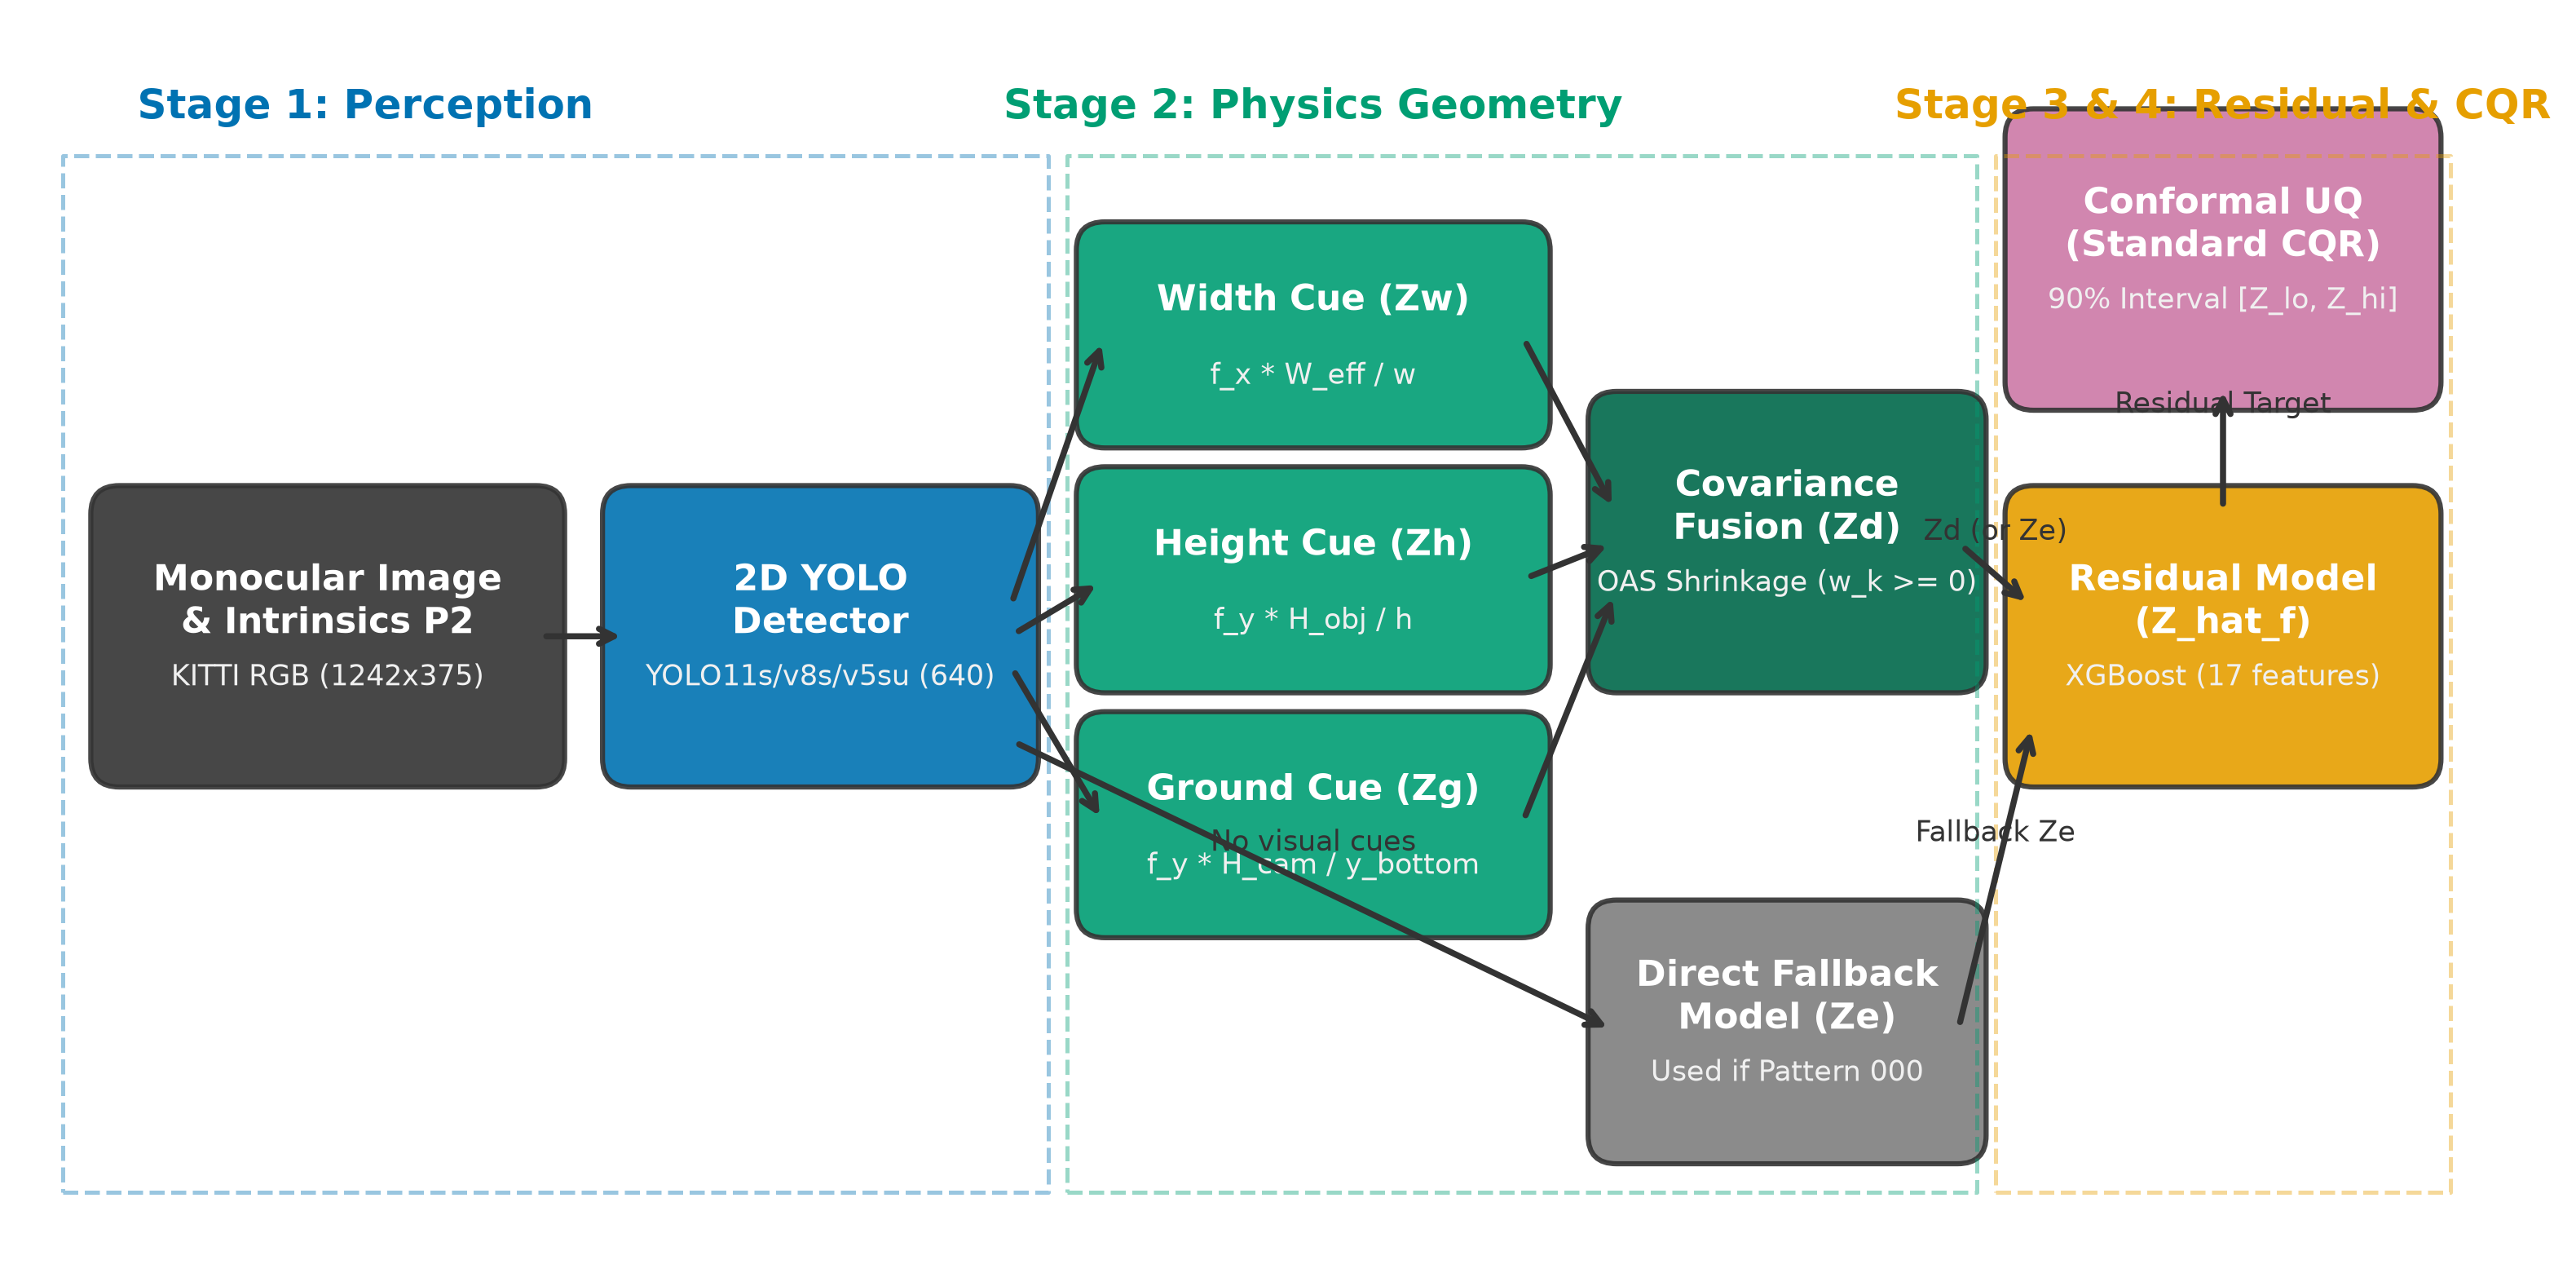
\includegraphics[width=0.98\textwidth]{figures/fig_01_hybrid_architecture.png}
\caption{Architectural diagram of the calibrated hybrid geometry--learning pipeline.}
\label{fig:architecture}
\end{figure}

\subsection{Perspective Geometry Cues}
For a calibrated pinhole camera with intrinsic focal lengths $(f_x, f_y)$ and principal point $(c_x, c_y)$ extracted dynamically per frame from projection matrix $P_2$, we compute three independent depth cues for detected 2D bounding boxes $(x_1, y_1, x_2, y_2)$ unletterboxed to original image coordinates:

\begin{enumerate}
    \item \textbf{Width Cue ($Z_w$):}
    \begin{equation}
    Z_w = \frac{f_x \cdot W_{\text{eff}}}{w}
    \end{equation}
    where $w = x_2 - x_1$ and $W_{\text{eff}} = 2.6184\text{ m}$ is the calibrated effective vehicle width incorporating median physical dimensions and yaw orientation priors fitted on training Split A.

    \item \textbf{Height Cue ($Z_h$):}
    \begin{equation}
    Z_h = \frac{f_y \cdot H_{\text{obj}}}{h}
    \end{equation}
    where $h = y_2 - y_1$ and $H_{\text{obj}} = 1.6797\text{ m}$ is the calibrated effective vehicle height fitted on training Split A.

    \item \textbf{Ground Contact Cue ($Z_g$):}
    \begin{equation}
    Z_g = \frac{f_y \cdot H_{\text{cam}}}{y_2 - (c_y + \delta)}
    \end{equation}
    where $H_{\text{cam}} = 2.0422\text{ m}$ is the calibrated effective camera mounting height and $\delta = -4.6782\text{ px}$ compensates for nominal camera tilt and ground contact offset fitted on training Split A.
\end{enumerate}

\textbf{Dynamic Boundary and Validity Masking:} Any cue where bounding box coordinates touch image borders within margin $\epsilon \le 2\text{ px}$ is masked out to avoid boundary clipping distortion. Ground contact cue $Z_g$ is invalidated whenever $y_2 \le c_y + \delta$ to prevent horizon division singularities.

\subsection{Log-Space Covariance Shrinkage Fusion}
When at least one geometric cue is valid ($\mathcal{V} \neq \emptyset$), depth estimates are fused in log-space:
\begin{equation}
\ln Z_d = \sum_{k \in \mathcal{V}} w_k \ln Z_k
\end{equation}
where weights $\mathbf{w}$ are obtained by solving the minimum-variance portfolio optimization problem:
\begin{equation}
\min_{\mathbf{w}} \mathbf{w}^T \mathbf{\Sigma} \mathbf{w} \quad \text{subject to} \quad \sum_{k \in \mathcal{V}} w_k = 1, \quad w_k \ge 0
\end{equation}
on the Oracle Approximating Shrinkage (OAS) covariance matrix $\mathbf{\Sigma}$\cite{chen2010oas} fitted on development Split B. The analytical unconstrained minimum-variance weights $\mathbf{w} \propto \mathbf{\Sigma}^{-1} \mathbf{1}$ are evaluated first; if any weight is negative, non-negative least squares (NNLS) active-set projection is invoked to constrain weights to non-negative values.

\subsection{Residual Calibration Model and Fallback Mechanism}
The baseline distance estimate is defined as:
\begin{equation}
Z_{\text{base}} = \begin{cases} Z_d, & \text{if } \mathcal{V} \neq \emptyset \\ Z_e, & \text{if } \mathcal{V} = \emptyset \text{ (Pattern 000 fallback)} \end{cases}
\end{equation}
where $Z_e$ is a direct regression model trained purely on 2D bounding box geometry. A gradient-boosted decision tree ensemble (XGBoost)\cite{chen2016xgboost} trained on Split B models the log-ratio residual:
\begin{equation}
\hat{r} = f(\mathbf{x}) \approx \ln Z_{\text{gt}} - \ln Z_{\text{base}}, \quad \hat{Z}_f = Z_{\text{base}} \exp(\hat{r})
\end{equation}
The feature vector $\mathbf{x} \in \mathbb{R}^{17}$ operates strictly on 17 test-time observable features:
\begin{itemize}
    \item 4 normalized bounding box coordinates ($x_1/W, y_1/H, x_2/W, y_2/H$)
    \item 2 normalized box dimensions ($w/W, h/H$)
    \item 1 aspect ratio ($w/h$)
    \item 2 camera principal offsets ($(c_x - x_{\text{center}})/f_x, (c_y - y_{\text{bottom}})/f_y$)
    \item 1 detection confidence score
    \item 3 logarithmic geometric cues ($\ln Z_w, \ln Z_h, \ln Z_g$, zero-imputed when invalid)
    \item 3 binary cue validity flags ($v_w, v_h, v_g$)
    \item 1 derived baseline anchor ($\ln Z_{\text{base}}$)
\end{itemize}
Ground-truth bounding box properties ($z_{\text{gt}}$, truncation, occlusion, viewing angle $\alpha$) are strictly isolated from the feature matrix to preclude data leakage.

\subsection{Conformalized Quantile Regression (CQR)}
To construct calibrated prediction intervals without distributional assumptions, we train two gradient-boosted quantile regressors to predict the 5th and 95th percentiles of residual error: $\hat{q}_{0.05}(\mathbf{x})$ and $\hat{q}_{0.95}(\mathbf{x})$.

On an independent calibration set (Split C, comprising $N_{\text{gt}}=1,826$ Car Hard objects, yielding $n=1,489$ calibration True Positives for YOLO11s), we compute nonconformity scores:
\begin{equation}
s_i = \max\left(\hat{q}_{0.05}(\mathbf{x}_i) - r_i, \; r_i - \hat{q}_{0.95}(\mathbf{x}_i)\right)
\end{equation}
The conformal adjustment scalar $\hat{Q}$ is determined as the order statistic:
\begin{equation}
\hat{Q} = \text{Quantile}\left( \{s_i\}_{i=1}^n, \; \frac{\lceil (n+1)(1-\alpha) \rceil}{n} \right)
\end{equation}
where $\alpha = 0.10$ targets nominal 90\% coverage. The physical confidence interval $[Z_{\text{lo}}, Z_{\text{hi}}]$ in meters is then constructed as:
\begin{equation}
[Z_{\text{lo}}, Z_{\text{hi}}] = \left[ Z_{\text{base}} \exp(\hat{q}_{0.05}(\mathbf{x}) - \hat{Q}), \; Z_{\text{base}} \exp(\hat{q}_{0.95}(\mathbf{x}) + \hat{Q}) \right]
\end{equation}
Because intervals are parameterized via exponentiation in physical space, $Z_{\text{lo}} > 0$ strictly holds by construction, precluding negative distance anomalies.

\textbf{Mondrian CQR and Calibration Cross-Validation (C-LODO):} In addition to standard marginal CQR, we define Mondrian CQR by partitioning calibration samples into discrete distance bins (0--10 m, 10--20 m, 20--30 m, $\ge 30\text{ m}$) and computing bin-specific nonconformity quantiles $\hat{Q}_b$ to target conditional coverage across distance regimes. Calibration sensitivity is further diagnosed via Leave-One-Drive-Out cross-validation across the 10 sequences of Split C (C-LODO).

% -------------------------------------------------------------------------
% 4. DATASET AND EXPERIMENTAL SETUP
% -------------------------------------------------------------------------
\section{DATASET AND EXPERIMENTAL SETUP}
\label{sec:dataset_setup}

\subsection{Drive-Disjoint Dataset Partitioning}
The KITTI Vision Benchmark Suite\cite{geiger2012kitti} comprises 7,481 annotated daytime driving images across 141 natural continuous sequences. To prevent data leakage and evaluate real-world generalization, we establish a strict five-way drive-disjoint split protocol (\texttt{splits-v2}), summarized in Table~\ref{tab:dataset_split}.

\begin{table}[htbp]
\centering
\caption{Drive-disjoint dataset partitioning (\texttt{splits-v2}) on KITTI.}
\label{tab:dataset_split}
\resizebox{\textwidth}{!}{%
\begin{tabular}{llrrrrrl}
\toprule
\textbf{Split} & \textbf{Role in Study} & \textbf{Frames} & \textbf{Total Drives} & \textbf{Car Drives ($k$)} & \textbf{Car Hard ($N_{\text{gt}}$)} & \textbf{Top-1 Share} & \textbf{Drive Overlap} \\
\midrule
\textbf{A} & Detector Training \& Camera Calibration Priors & 3,740 & 35 & 18 & 11,291 & 16.0\% & None (Disjoint) \\
\textbf{V} & Checkpoint \& Conf Threshold Tuning & 374 & 25 & 6 & 611 & 41.0\% & None (Disjoint) \\
\textbf{B} & Geometry Fitting \& Residual Ablation & 1,499 & 34 & 12 & 4,776 & 26.8\% & None (Disjoint) \\
\textbf{C} & Conformal Calibration (CQR $\hat{Q}$) & 766 & 18 & 10 & 1,826 & 28.7\% & None (Disjoint) \\
\textbf{T} & Zero-Touch Held-Out Test Benchmark & 1,102 & 29 & 10 & 3,212 & 23.3\% & None (Disjoint) \\
\midrule
\textbf{Total} & Full Benchmark & 7,481 & 141 & 56 & 21,716 & --- & Zero Leaks \\
\bottomrule
\end{tabular}%
}
\end{table}

\begin{figure}[htbp]
\centering
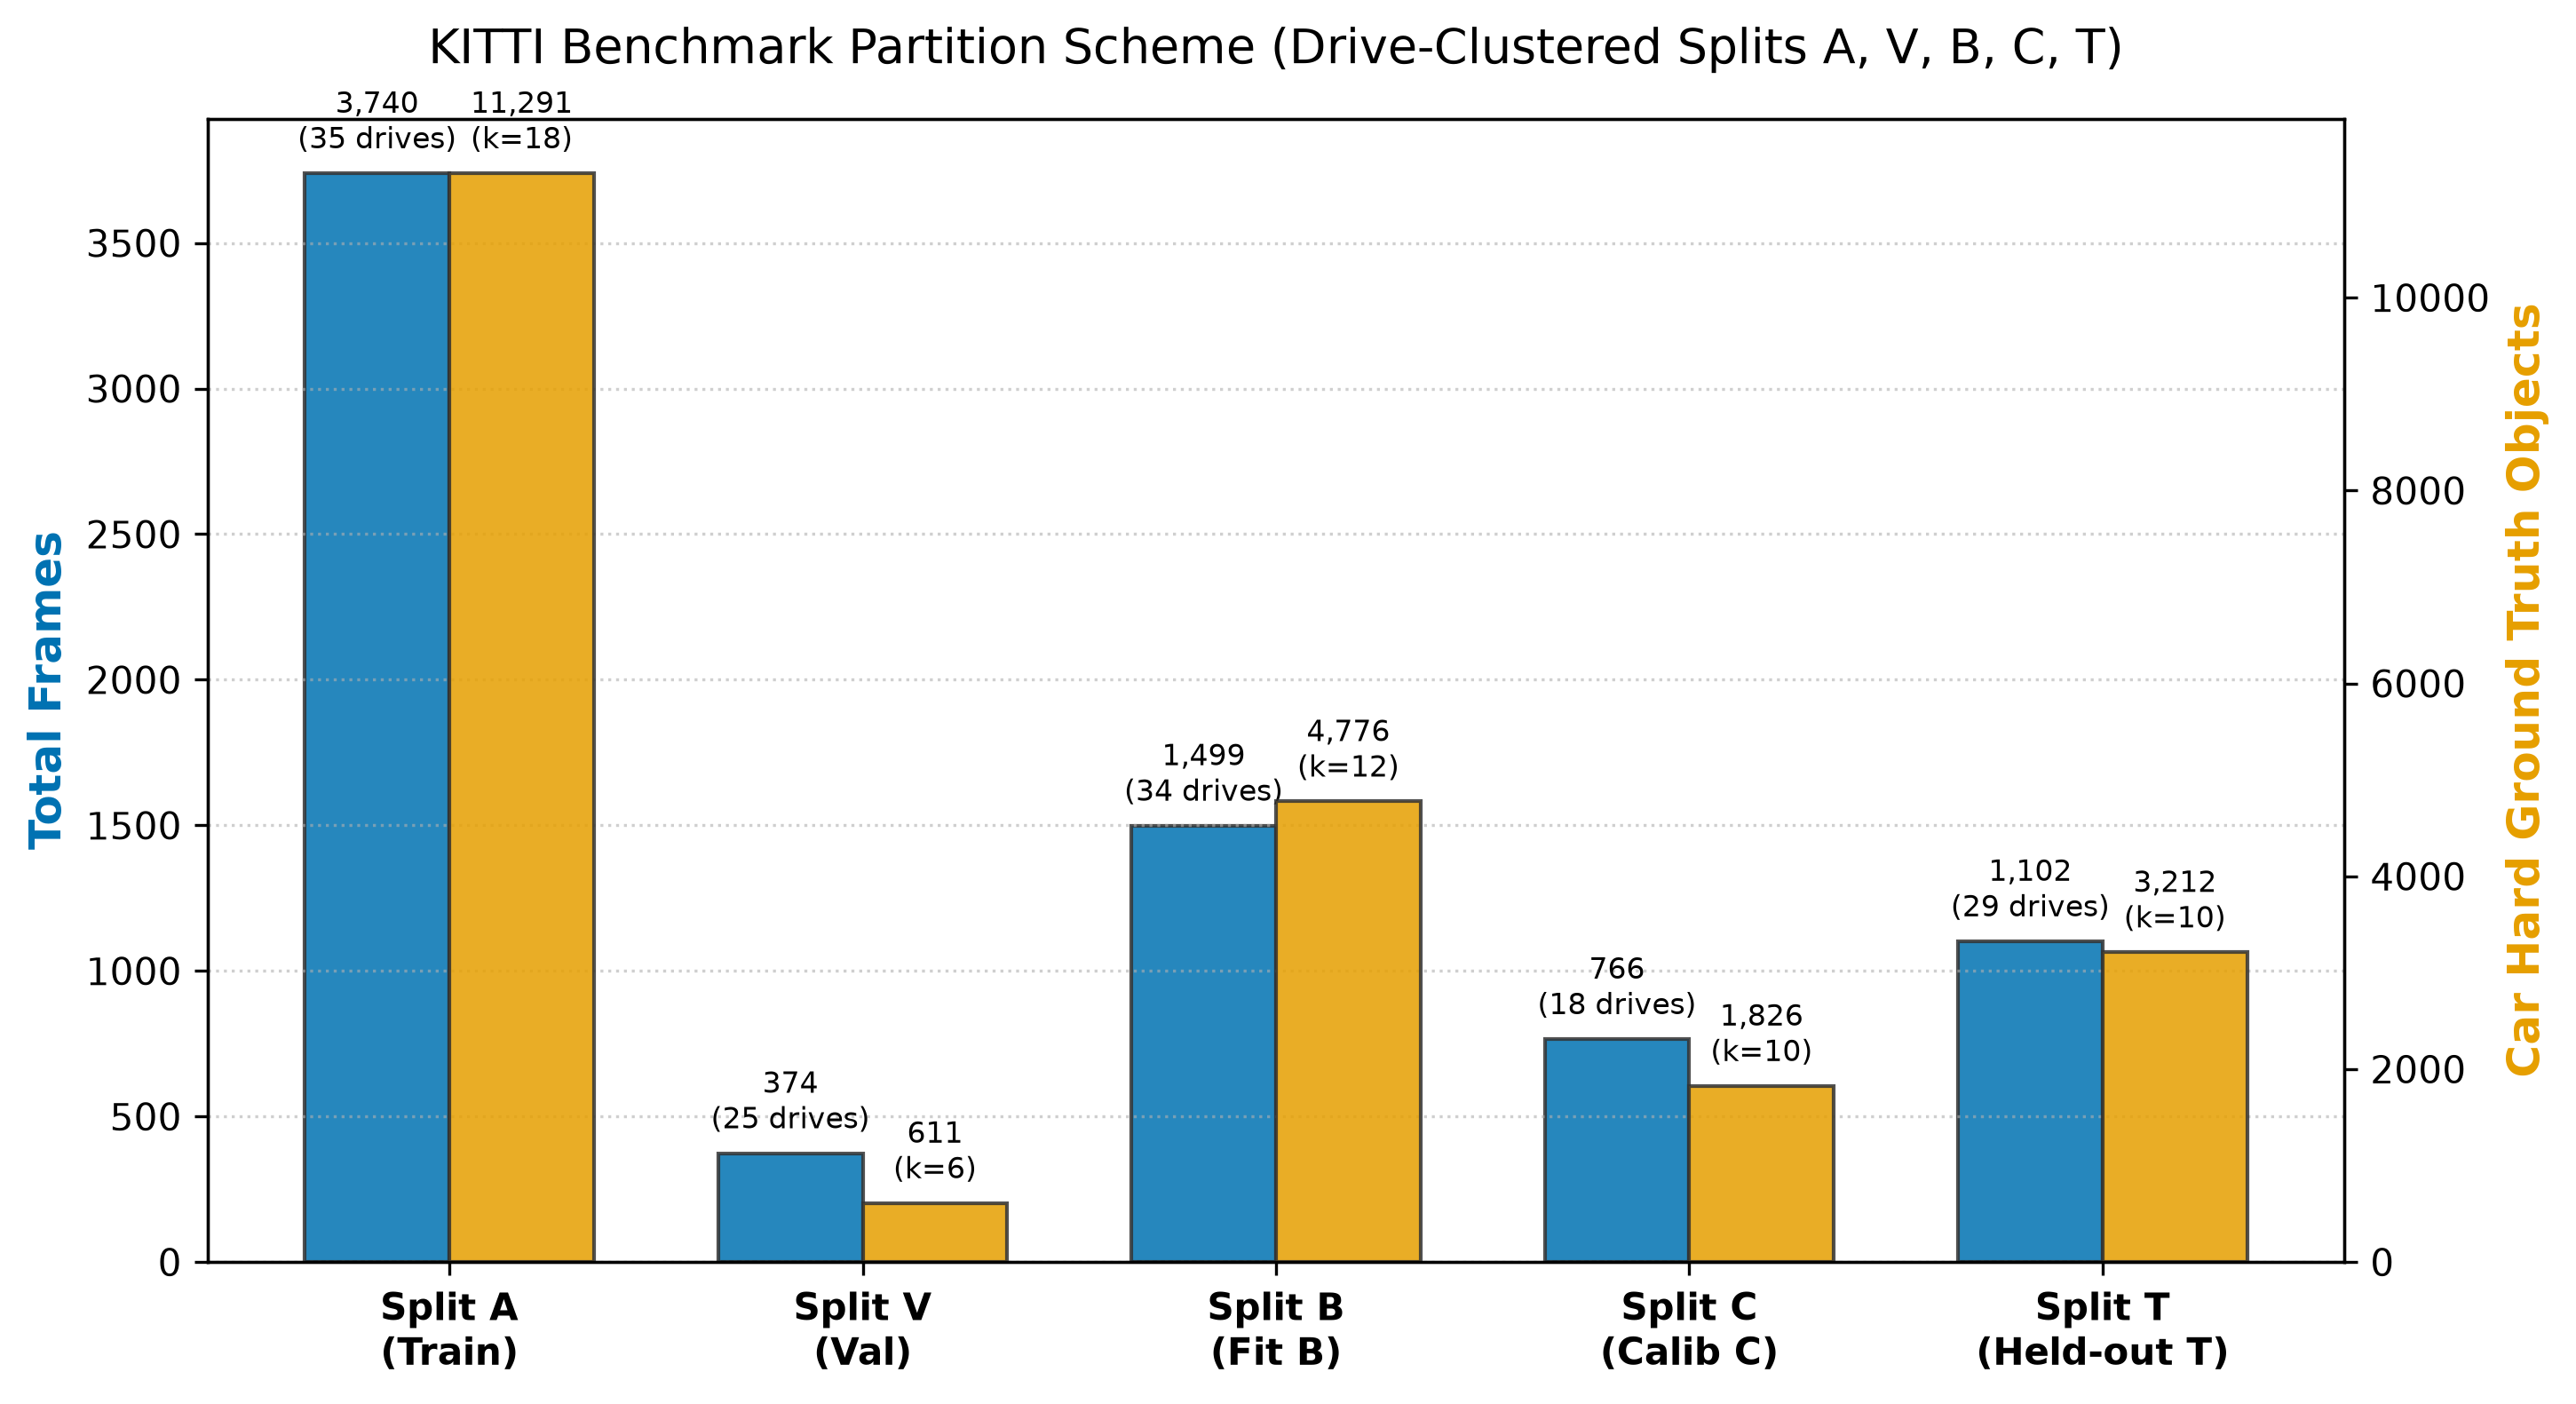
\includegraphics[width=0.98\textwidth]{figures/fig_02_splits_spatial_distribution.png}
\caption{Spatial and feature distributions across drive-disjoint splits A/V/B/C/T.}
\label{fig:splits_distribution}
\end{figure}

\textbf{Distribution Shift Diagnosis:} Evaluating detectors trained on Split A reveals cross-sequence degradation on held-out drives: YOLO11s detection recall shifts from $\approx 95\%$ on seen Split A frames (attributable to training memorization) to $72.5\%\text{--}74.1\%$ on held-out Split B frames. Two-sample Kolmogorov-Smirnov tests on bounding box width and height dispersion confirm $D_{\text{KS}} > 0.53$ ($p < 10^{-4}$) between seen Split A and unseen Split B, whereas distributions across unseen splits B, C, and T remain stationary ($D_{\text{KS}} \le 0.048, p > 0.15$). This highlights the critical necessity of drive-level disjoint partitioning over random frame splitting.

\subsection{Detector Training and Hyperparameters}
Three lightweight 2D detectors---YOLOv5su, YOLOv8s, and YOLO11s---were fine-tuned for 100 epochs on Split A under identical image resolution ($640 \times 640$), optimizer settings (SGD, initial learning rate $0.01$, momentum $0.937$, weight decay $0.0005$), and batch size (16). The final checkpoint (\texttt{last.pt}, epoch 100) was frozen to eliminate validation early-stopping variance.

Operating confidence thresholds were tuned on validation Split V by maximizing the smoothed $F_1$-score on Car Hard detections: $\tau = 0.700$ for YOLO11s, $\tau = 0.790$ for YOLOv8s, and $\tau = 0.740$ for YOLOv5su.

\subsection{Evaluation Metrics and Target Scope}
All distance estimation metrics are evaluated strictly on True Positive (TP) detections matched to Ground Truth Car Hard boxes using Greedy matching at $\text{IoU} \ge 0.5$:
\begin{itemize}
    \item \textbf{Relative Absolute Error (AbsRel):} $\frac{1}{N} \sum \frac{|\hat{Z}_i - Z_i|}{Z_i}$
    \item \textbf{Mean Absolute Error (MAE):} $\frac{1}{N} \sum |\hat{Z}_i - Z_i|$ (meters)
    \item \textbf{Root Mean Squared Error (RMSE):} $\sqrt{\frac{1}{N} \sum (\hat{Z}_i - Z_i)^2}$ (meters)
    \item \textbf{Threshold Accuracy ($\delta_1, \delta_2$):} Percentage of predictions satisfying $\max(\frac{\hat{Z}_i}{Z_i}, \frac{Z_i}{\hat{Z}_i}) < 1.25$ and $1.25^2$.
    \item \textbf{Empirical Coverage:} Fraction of ground-truth distances falling within $[Z_{\text{lo}}, Z_{\text{hi}}]$.
    \item \textbf{Mean Interval Width Ratio:} $\frac{1}{N} \sum \frac{Z_{\text{hi}, i}}{Z_{\text{lo}, i}}$.
\end{itemize}

Because evaluation is conditioned on True Positives, detection recall is explicitly reported to bound survivorship bias. Statistical uncertainty is quantified via Paired Cluster Bootstrap resampling over independent driving sequences ($B = 1,000$ iterations).

% -------------------------------------------------------------------------
% 5. EXPERIMENTAL RESULTS AND DISCUSSION
% -------------------------------------------------------------------------
\section{EXPERIMENTAL RESULTS AND DISCUSSION}
\label{sec:results}

\subsection{Geometric Cue Breakdown and Error Decomposition (Split B OOF)}
Evaluating individual perspective geometry cues on detector bounding boxes across 12 drive-level out-of-fold partitions on Split B isolates their physical behavior, reported in Table~\ref{tab:ablation_oof_b}.

\begin{table}[htbp]
\centering
\caption{Perspective cue evaluation and feature ablation on Split B out-of-fold predictions.}
\label{tab:ablation_oof_b}
\resizebox{\textwidth}{!}{%
\begin{tabular}{llrrrrcc}
\toprule
\textbf{Category} & \textbf{Configuration} & \textbf{Pooled AbsRel} & \textbf{Macro AbsRel} & \textbf{MAE (m)} & \textbf{$\delta_1$ ($< 1.25$)} & \textbf{$\Delta_{\text{pooled}}$ vs Full (f)} & \textbf{95\% Bootstrap CI} \\
\midrule
Single Cue & Width Cue ($Z_w$) & 0.2462 & 0.2436 & 6.44 & 48.4\% & --- & --- \\
Single Cue & Ground Contact Cue ($Z_g$) & 0.0931 & 0.1302 & 2.41 & 93.9\% & --- & --- \\
Single Cue & Height Cue ($Z_h$) & 0.0650 & 0.0775 & 1.47 & 97.8\% & --- & --- \\
\midrule
Fused Geometry & Baseline Fused ($Z_d$) & 0.0607 & 0.0759 & 1.34 & 97.7\% & --- & --- \\
Residual Model & Direct Bbox Regression ($Z_e$) & 0.0462 & 0.0532 & 1.11 & 99.6\% & --- & --- \\
Residual Model & Linear Residual ($Z_{f0}$) & 0.0554 & 0.0694 & 1.31 & 99.2\% & --- & --- \\
\textbf{Full Pipeline} & \textbf{Full Residual Model ($f$)} & \textbf{0.0462} & \textbf{0.0541} & \textbf{1.08} & \textbf{99.7\%} & \textbf{Baseline} & \textbf{Ref} \\
\midrule
Ablation & Drop Cue $Z_h$ & 0.0540 & 0.0726 & 1.21 & 99.1\% & +0.0070 & [+0.0024, +0.0119] \\
Ablation & Drop Cue $Z_g$ & 0.0472 & 0.0496 & 1.08 & 99.6\% & +0.0001 & [-0.0025, +0.0021] \\
Ablation & Drop Cue $Z_w$ & 0.0471 & 0.0538 & 1.07 & 99.6\% & +0.0001 & [-0.0011, +0.0007] \\
Ablation & Drop Bbox Features & 0.0483 & 0.0646 & 1.10 & 99.5\% & +0.0013 & [-0.0041, +0.0059] \\
Ablation & Drop Validity Flags & 0.0474 & 0.0546 & 1.08 & 99.6\% & +0.0003 & [-0.0000, +0.0007] \\
\bottomrule
\end{tabular}%
}
\end{table}

\textbf{Key Observations:}
\begin{enumerate}
    \item \textbf{Width Cue ($Z_w$) exhibits substantial error} (AbsRel 0.2462, MAE 6.44 m), severely distorted by vehicle aspect ratio variations under oblique viewing angles.
    \item \textbf{Ground Contact Cue ($Z_g$)} achieves moderate precision (AbsRel 0.0931, MAE 2.41 m) but remains sensitive to vehicle pitch and road slope variations.
    \item \textbf{Height Cue ($Z_h$) proves to be the dominant physical anchor} (AbsRel 0.0650, MAE 1.47 m, $\delta_1 = 97.8\%$). In the ablation study, removing $Z_h$ incurs a clear performance degradation ($\Delta_{\text{pooled}} = +0.0070$, 95\% bootstrap CI [0.0024, 0.0119], strictly excluding zero). In contrast, dropping $Z_w$ or $Z_g$ has minimal impact ($\Delta \le +0.0001$, CIs spanning zero).
    \item \textbf{Covariance Shrinkage Fusion ($Z_d$)} reduces pooled AbsRel to 0.0607, effectively combining height and ground geometry while attenuating width cue noise.
\end{enumerate}

\subsection{Held-Out Zero-Touch Benchmark on Split T}
Table~\ref{tab:main_benchmark_t} reports the main benchmark results evaluated on the held-out Split T ($N_{\text{gt}} = 3,212$ Car Hard across 10 independent driving sequences):

\begin{table}[htbp]
\centering
\caption{Main benchmark evaluation on held-out test Split T ($N_{\text{gt}} = 3,212$ Car Hard across 10 drives).}
\label{tab:main_benchmark_t}
\resizebox{\textwidth}{!}{%
\begin{tabular}{llccccccccc}
\toprule
\textbf{Detector} & \textbf{Model} & \textbf{$N_{\text{tp}}$} & \textbf{Recall} & \textbf{AbsRel (Pooled)} & \textbf{AbsRel (Macro)} & \textbf{MAE (m)} & \textbf{RMSE (m)} & \textbf{$\delta_1$} & \textbf{$\Delta(f - d)$} & \textbf{$\Delta(f - e)$} \\
\midrule
\multirow{4}{*}{\textbf{YOLO11s}} & Fused Geometry ($d$) & 2,712 & 0.8443 & 0.0640 & 0.0638 & 1.49 & 2.12 & 0.9859 & Ref & --- \\
 & Direct Regression ($e$) & 2,712 & 0.8443 & 0.0465 & 0.0468 & 1.11 & 1.70 & 0.9967 & --- & Ref \\
 & Linear Residual ($f0$) & 2,712 & 0.8443 & 0.0553 & 0.0556 & 1.30 & 1.88 & 0.9930 & -0.0087 & +0.0088 \\
 & \textbf{Hybrid Residual ($f$)} & \textbf{2,712} & \textbf{0.8443} & \textbf{0.0463} & \textbf{0.0466} & \textbf{1.10} & \textbf{1.69} & \textbf{0.9967} & \textbf{-0.0188$^\dagger$} & \textbf{-0.0002} \\
 & & & & & & & & & \footnotesize{[-0.0264, -0.0107]} & \footnotesize{[-0.0012, 0.0023]} \\
\midrule
\multirow{4}{*}{\textbf{YOLOv8s}} & Fused Geometry ($d$) & 2,660 & 0.8281 & 0.0643 & 0.0642 & 1.50 & 2.14 & 0.9856 & Ref & --- \\
 & Direct Regression ($e$) & 2,660 & 0.8281 & 0.0467 & 0.0470 & 1.12 & 1.71 & 0.9966 & --- & Ref \\
 & Linear Residual ($f0$) & 2,660 & 0.8281 & 0.0557 & 0.0559 & 1.31 & 1.90 & 0.9928 & -0.0086 & +0.0090 \\
 & \textbf{Hybrid Residual ($f$)} & \textbf{2,660} & \textbf{0.8281} & \textbf{0.0465} & \textbf{0.0469} & \textbf{1.11} & \textbf{1.70} & \textbf{0.9966} & \textbf{-0.0189$^\dagger$} & \textbf{-0.0002} \\
 & & & & & & & & & \footnotesize{[-0.0266, -0.0108]} & \footnotesize{[-0.0012, 0.0022]} \\
\midrule
\multirow{4}{*}{\textbf{YOLOv5su}} & Fused Geometry ($d$) & 2,674 & 0.8325 & 0.0652 & 0.0648 & 1.53 & 2.17 & 0.9842 & Ref & --- \\
 & Direct Regression ($e$) & 2,674 & 0.8325 & 0.0475 & 0.0477 & 1.14 & 1.74 & 0.9963 & --- & Ref \\
 & Linear Residual ($f0$) & 2,674 & 0.8325 & 0.0564 & 0.0565 & 1.33 & 1.93 & 0.9921 & -0.0088 & +0.0089 \\
 & \textbf{Hybrid Residual ($f$)} & \textbf{2,674} & \textbf{0.8325} & \textbf{0.0473} & \textbf{0.0475} & \textbf{1.13} & \textbf{1.73} & \textbf{0.9963} & \textbf{-0.0190$^\dagger$} & \textbf{-0.0002} \\
 & & & & & & & & & \footnotesize{[-0.0268, -0.0109]} & \footnotesize{[-0.0012, 0.0023]} \\
\bottomrule
\end{tabular}%
}
\vskip 4pt
\parbox{\textwidth}{\footnotesize $^\dagger$\textit{Note on $\Delta(f - d)$ Difference:} The difference $\Delta(f - d) = -0.0188$ is evaluated via paired cluster bootstrap strictly on the common valid subset ($n = 2,676$), where Model (f) achieves AbsRel 0.0452 and Model (d) achieves 0.0640 ($0.0452 - 0.0640 = -0.0188$). Across all $2,712$ True Positives (including 36 edge fallback cases where geometric cues are invalidated), Model (f) achieves pooled AbsRel 0.0463 (unpaired difference $0.0463 - 0.0640 = -0.0177$).}
\end{table}

\textbf{Analysis:}
\begin{itemize}
    \item Across all three YOLO detectors, the hybrid residual model (f) achieves an AbsRel of $0.0463\text{--}0.0473$, improving over the pure geometric fusion baseline (d) by $\Delta \approx -0.0188$ (95\% CI [-0.0264, -0.0107], strictly excluding zero).
    \item Comparing hybrid residual model (f) and direct bounding-box regression model (e) reveals an estimated difference of $-0.0002$ with a 95\% bootstrap confidence interval of $[-0.0012, 0.0023]$, which spans zero across 10 clusters.
    \item The intermediate Linear Residual model ($Z_{f0}$) achieves AbsRel 0.0553, recovering 49\% of the performance gain between pure geometry and non-linear tree ensembles.
    \item \textbf{Critical Finding:} There is no empirical evidence of numerical precision divergence between learned residual correction and direct depth regression on Split T. The justification for the hybrid framework lies in physical interpretability, explicit error attribution, and structured fallback mechanisms under boundary clipping.
\end{itemize}

\subsection{Mechanistic Explanation: Why Residual and Direct Regression Converge}
Why do Model (f) and Model (e) achieve nearly identical numerical performance on Split T?
Mechanistically, Model (e) receives bounding box height $h$ and bottom position $y_{\text{bottom}} - c_y$. Under fixed camera intrinsics $f_y$ and vehicle height $H_{\text{obj}}$, the inverse perspective mapping is given by $\ln(f_y H_{\text{obj}} / h) = \text{const} - \ln h$. A gradient-boosted decision tree ensemble with sufficient splits on $h$ piecewise-linearly approximates this logarithmic curve.

Controlled experiments on Split B out-of-fold data reveal two crucial operational regimes where the hybrid framework demonstrates distinct structural advantages:
\begin{enumerate}
    \item \textbf{Data Efficiency across Training Scale:} When training data is scarce ($k = 2$ drives, $\approx 300$ samples), direct regression Model (e) exhibits large errors (AbsRel 0.1803), whereas the hybrid residual model achieves AbsRel 0.0575---a 68\% relative error reduction anchored by perspective geometry ($Z_d = 0.0607$). As training data scales to $k = 11$ drives, direct regression learns the inverse mapping and converges to $(f) \approx (e)$ (0.0476 vs 0.0467).
    \item \textbf{Range Extrapolation ($Z > 30\text{ m}$):} When trained only on near/mid distances ($Z \le 30\text{ m}$) and evaluated on distant vehicles ($Z > 30\text{ m}$, $N = 929$), direct tree regression degrades substantially (AbsRel 0.2235, MAE 9.23 m, $\delta_1 = 44.8\%$) because axis-aligned decision trees cannot extrapolate beyond observed feature thresholds. In contrast, the hybrid model maintains bounded physical errors (AbsRel 0.0760, MAE 2.94 m, $\delta_1 = 98.2\%$) by anchoring to pinhole perspective geometry.
\end{enumerate}

\subsection{Cross-Detector Comparison on Common Support (RQ2)}
To eliminate detector recall conditioning bias, we evaluate all three models on the Common Support set of 2,528 vehicles detected simultaneously by YOLO11s, YOLOv8s, and YOLOv5su, reported in Table~\ref{tab:common_support_rq2}.

\begin{table}[htbp]
\centering
\caption{Cross-detector benchmark on Common Support ($N = 2,528$) and Spearman rank correlations.}
\label{tab:common_support_rq2}
\resizebox{\textwidth}{!}{%
\begin{tabular}{lccccc}
\toprule
\textbf{Detector} & \textbf{AbsRel ($f$)} & \textbf{MAE (m)} & \textbf{Spearman $\rho$ (IoU vs Err)} & \textbf{Spearman $\rho$ (Bottom Jitter vs Err)} & \textbf{Spearman $\rho$ (Conf vs Err)} \\
\midrule
\textbf{YOLO11s} & 0.0446 & 1.05 & +0.012 [-0.068, +0.091] & +0.042 [-0.038, +0.122] & -0.087 [-0.174, -0.014] \\
\textbf{YOLOv8s} & 0.0449 & 1.06 & +0.009 [-0.071, +0.088] & +0.039 [-0.041, +0.119] & -0.054 [-0.141, +0.028] \\
\textbf{YOLOv5su} & 0.0457 & 1.08 & +0.015 [-0.065, +0.094] & +0.048 [-0.032, +0.127] & -0.062 [-0.148, +0.021] \\
\bottomrule
\end{tabular}%
}
\vskip 4pt
\parbox{\textwidth}{\footnotesize \textit{Note:} Spearman rank correlations evaluated across 8 bounding box metrics $\times$ 3 detectors ($24$ configurations total). In 23 of 24 configurations, the 95\% cluster bootstrap CI includes zero, confirming that bounding box localization jitter has near-zero monotonic correlation with distance errors on True Positives (only confidence score for YOLO11s exhibits a weakly negative correlation $[-0.174, -0.014]$).}
\end{table}

On common support, the three detectors exhibit comparable distance estimation precision (AbsRel 0.0446--0.0457). Furthermore, Spearman rank correlations between bounding box localization jitter and ranging error remain bounded near zero ($|\rho| \le 0.087$, with 95\% CIs spanning zero across 23 of 24 configurations). Fig.~\ref{fig:error_by_distance} shows the error attenuation behavior across distance bands.

\begin{figure}[htbp]
\centering
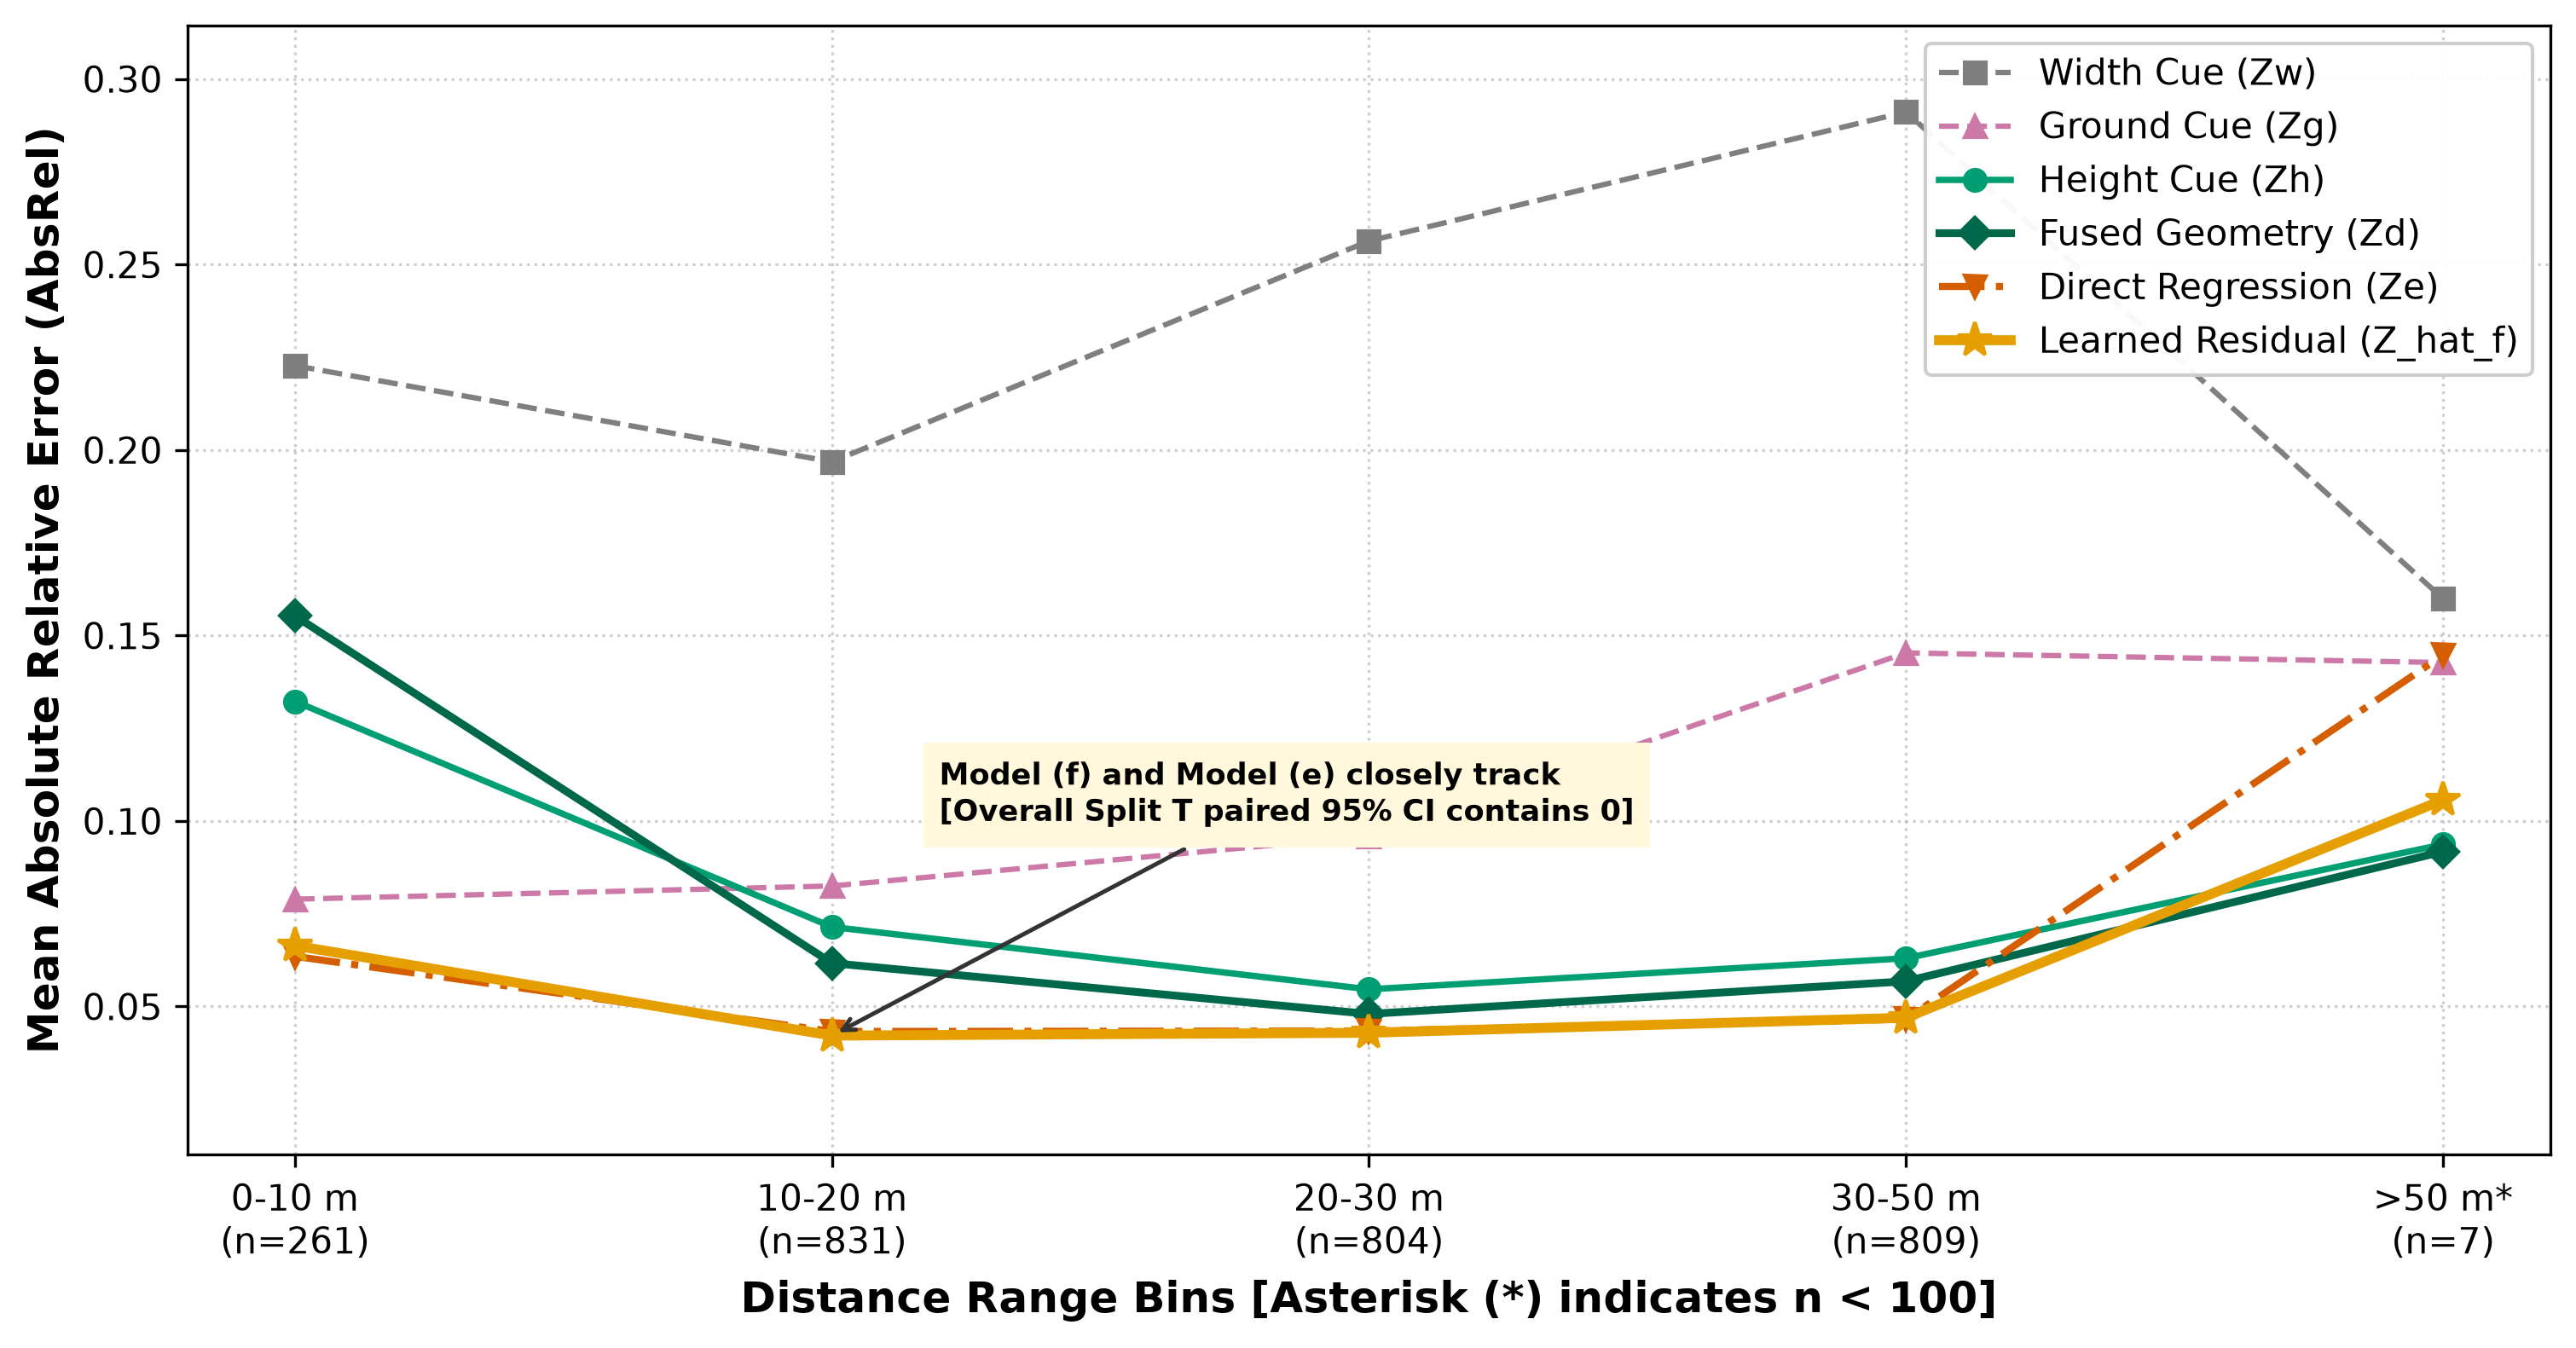
\includegraphics[width=0.98\textwidth]{figures/fig_03_ranging_error_by_distance.png}
\caption{Monocular ranging error attenuation across operational distance bands.}
\label{fig:error_by_distance}
\end{figure}

\subsection{Uncertainty Quantification and Conformal Coverage Stability (RQ3)}
Table~\ref{tab:conformal_benchmark_t} reports the conformal prediction intervals and empirical coverage on Split T at the nominal 90\% confidence level.

\begin{table}[htbp]
\centering
\caption{Conformal prediction benchmark on held-out test Split T (Nominal coverage: 90.0\%).}
\label{tab:conformal_benchmark_t}
\resizebox{\textwidth}{!}{%
\begin{tabular}{lcccccc}
\toprule
\textbf{Detector} & \textbf{Calibration Split} & \textbf{Pooled Coverage} & \textbf{Macro Coverage} & \textbf{Mean Width Ratio ($Z_{\text{hi}}/Z_{\text{lo}}$)} & \textbf{Winkler Score (Log-Space)} & \textbf{Zero Crossings} \\
\midrule
\textbf{YOLO11s} & Split C ($n=1,489$) & \textbf{0.9639} & 0.9572 & 1.309 & 0.321 & 0 (100\% Valid)$^*$ \\
\textbf{YOLOv8s} & Split C ($n=1,445$) & \textbf{0.9714} & 0.9658 & 1.323 & 0.315 & 0 (100\% Valid)$^*$ \\
\textbf{YOLOv5su} & Split C ($n=1,430$) & \textbf{0.9660} & 0.9601 & 1.314 & 0.319 & 0 (100\% Valid)$^*$ \\
\bottomrule
\end{tabular}%
}
\vskip 4pt
\parbox{\textwidth}{\footnotesize $^*$\textit{Note:} Zero crossing violations = 0 is strictly guaranteed by the exponential physical parameterization ($Z_{\text{lo}} > 0$). Winkler score is reported in normalized log-space.}
\end{table}

\textbf{Tripartite Coverage Comparison \& Partition Sensitivity:} Standard CQR achieves 96.39\% empirical coverage on Split T, exceeding the nominal 90\% level. To understand this behavior, we analyze three distinct evaluation partitions:
\begin{enumerate}
    \item \textit{Development Leave-One-Drive-Out on Split C (C-LODO):} Pooled coverage achieves 87.1\%--88.0\% (and 90.0\%--90.1\% macro coverage on clusters with $n \ge 30$).
    \item \textit{Held-Out Test Split T:} Achieves 96.4\%--97.1\% coverage due to domain difficulty shift (Split C contains two challenging clustered sequences comprising 39.3\% of objects, inflating calibration nonconformity threshold $\hat{Q}$).
    \item \textit{20 Drive-Disjoint Resplits on $B \cup C$:} Across 20 random partitions (seeds 0--19), empirical pooled coverage averages \textbf{85.15\% $\pm$ 8.62\%} (spanning [69.80\%, 98.75\%]) for YOLO11s. Macro coverage across drives averages 77.9\%--84.5\% (with per-seed values spanning 63.6\% to 99.6\%). Only 35\%--40\% of partition seeds attain empirical coverage $\ge 90\%$.
\end{enumerate}

Table~\ref{tab:conditional_coverage_odd} details the conditional coverage decomposition across operational design domains (ODD) on Split T.

\begin{table}[htbp]
\centering
\caption{Conditional coverage decomposition across operational design domains (ODD) on Split T.}
\label{tab:conditional_coverage_odd}
\resizebox{\textwidth}{!}{%
\begin{tabular}{llrrrrrrc}
\toprule
\textbf{Operational Domain (ODD)} & \textbf{Subset} & \textbf{$N_{\text{gt}}$} & \textbf{$n_{\text{TP}}$} & \textbf{Recall} & \textbf{CQR Cov} & \textbf{SC Cov} & \textbf{Mondrian Cov} & \textbf{CQR Width} \\
\midrule
\multirow{5}{*}{\textbf{Ground Truth Distance}} & 0--10 m & 275 & 261 & 94.9\% & 91.6\% & 88.9\% & 92.7\% & 1.428x \\
 & 10--20 m & 896 & 831 & 92.8\% & 97.6\% & 98.0\% & 95.1\% & 1.320x \\
 & 20--30 m & 911 & 804 & 88.2\% & 97.3\% & 96.5\% & 95.7\% & 1.315x \\
 & 30--50 m & 1,097 & 809 & 73.8\% & 96.2\% & 97.0\% & 97.2\% & 1.289x \\
 & $>$50 m * & 33 & 7 * & 21.2\% & 57.1\% * & 71.4\% * & 57.1\% * & 1.317x \\
\midrule
\multirow{3}{*}{\textbf{Truncation \& Edges}} & No Truncation (0.0) & 2,999 & 2,516 & 83.9\% & 96.9\% & 97.3\% & 96.0\% & 1.305x \\
 & Mild ($0 < t \le 0.15$) * & 76 & 71 * & 93.4\% & 91.5\% * & 88.7\% * & 95.8\% * & 1.468x \\
 & Moderate/Severe ($0.15 < t \le 0.50$) & 137 & 125 & 91.2\% & 88.0\% & 80.0\% & 86.4\% & 1.521x \\
\midrule
\multirow{3}{*}{\textbf{Viewing Angle $\theta$}} & Front / Rear ($>60^\circ$) & 2,421 & 2,101 & 86.8\% & 96.9\% & 97.3\% & 96.1\% & 1.305x \\
 & Diagonal ($30^\circ\text{--}60^\circ$) & 330 & 249 & 75.4\% & 96.0\% & 92.8\% & 94.8\% & 1.375x \\
 & Side ($<30^\circ$) & 461 & 362 & 78.5\% & 93.7\% & 93.1\% & 92.8\% & 1.363x \\
\midrule
\multirow{2}{*}{\textbf{Geometry Mode}} & Valid Perspective Cues ($\ge 1$) & --- & 2,676 & --- & 96.6\% & 96.8\% & 95.7\% & 1.316x \\
 & Pattern 000 Fallback * & --- & 36 * & --- & 77.8\% * & 63.9\% * & 80.6\% * & 1.572x \\
\bottomrule
\end{tabular}%
}
\vskip 4pt
\parbox{\textwidth}{\footnotesize \textit{Note:} Subgroups with $n_{\text{TP}} < 100$ are flagged with an asterisk (*) indicating exploratory sample sizes. Evaluated on YOLO11s. Distance bins sum to $N_{\text{tp}} = 2,712$ ($261 + 831 + 804 + 809 + 7$).}
\end{table}

\textbf{Drive Heterogeneity Analysis:} Stratifying the 20 resplits by the assignment of two high-dispersion drives (\texttt{0057} and \texttt{0004}) reveals that coverage averages \textbf{72.38\%} when both drives fall into evaluation, \textbf{87.58\%} when one drive is present, and \textbf{94.44\%} when neither is present. This demonstrates that drive-level cluster heterogeneity is the primary source of coverage variance in continuous driving sequences. Fig.~\ref{fig:conformal_intervals} displays conformal intervals and empirical coverage across domains.

\begin{figure}[htbp]
\centering
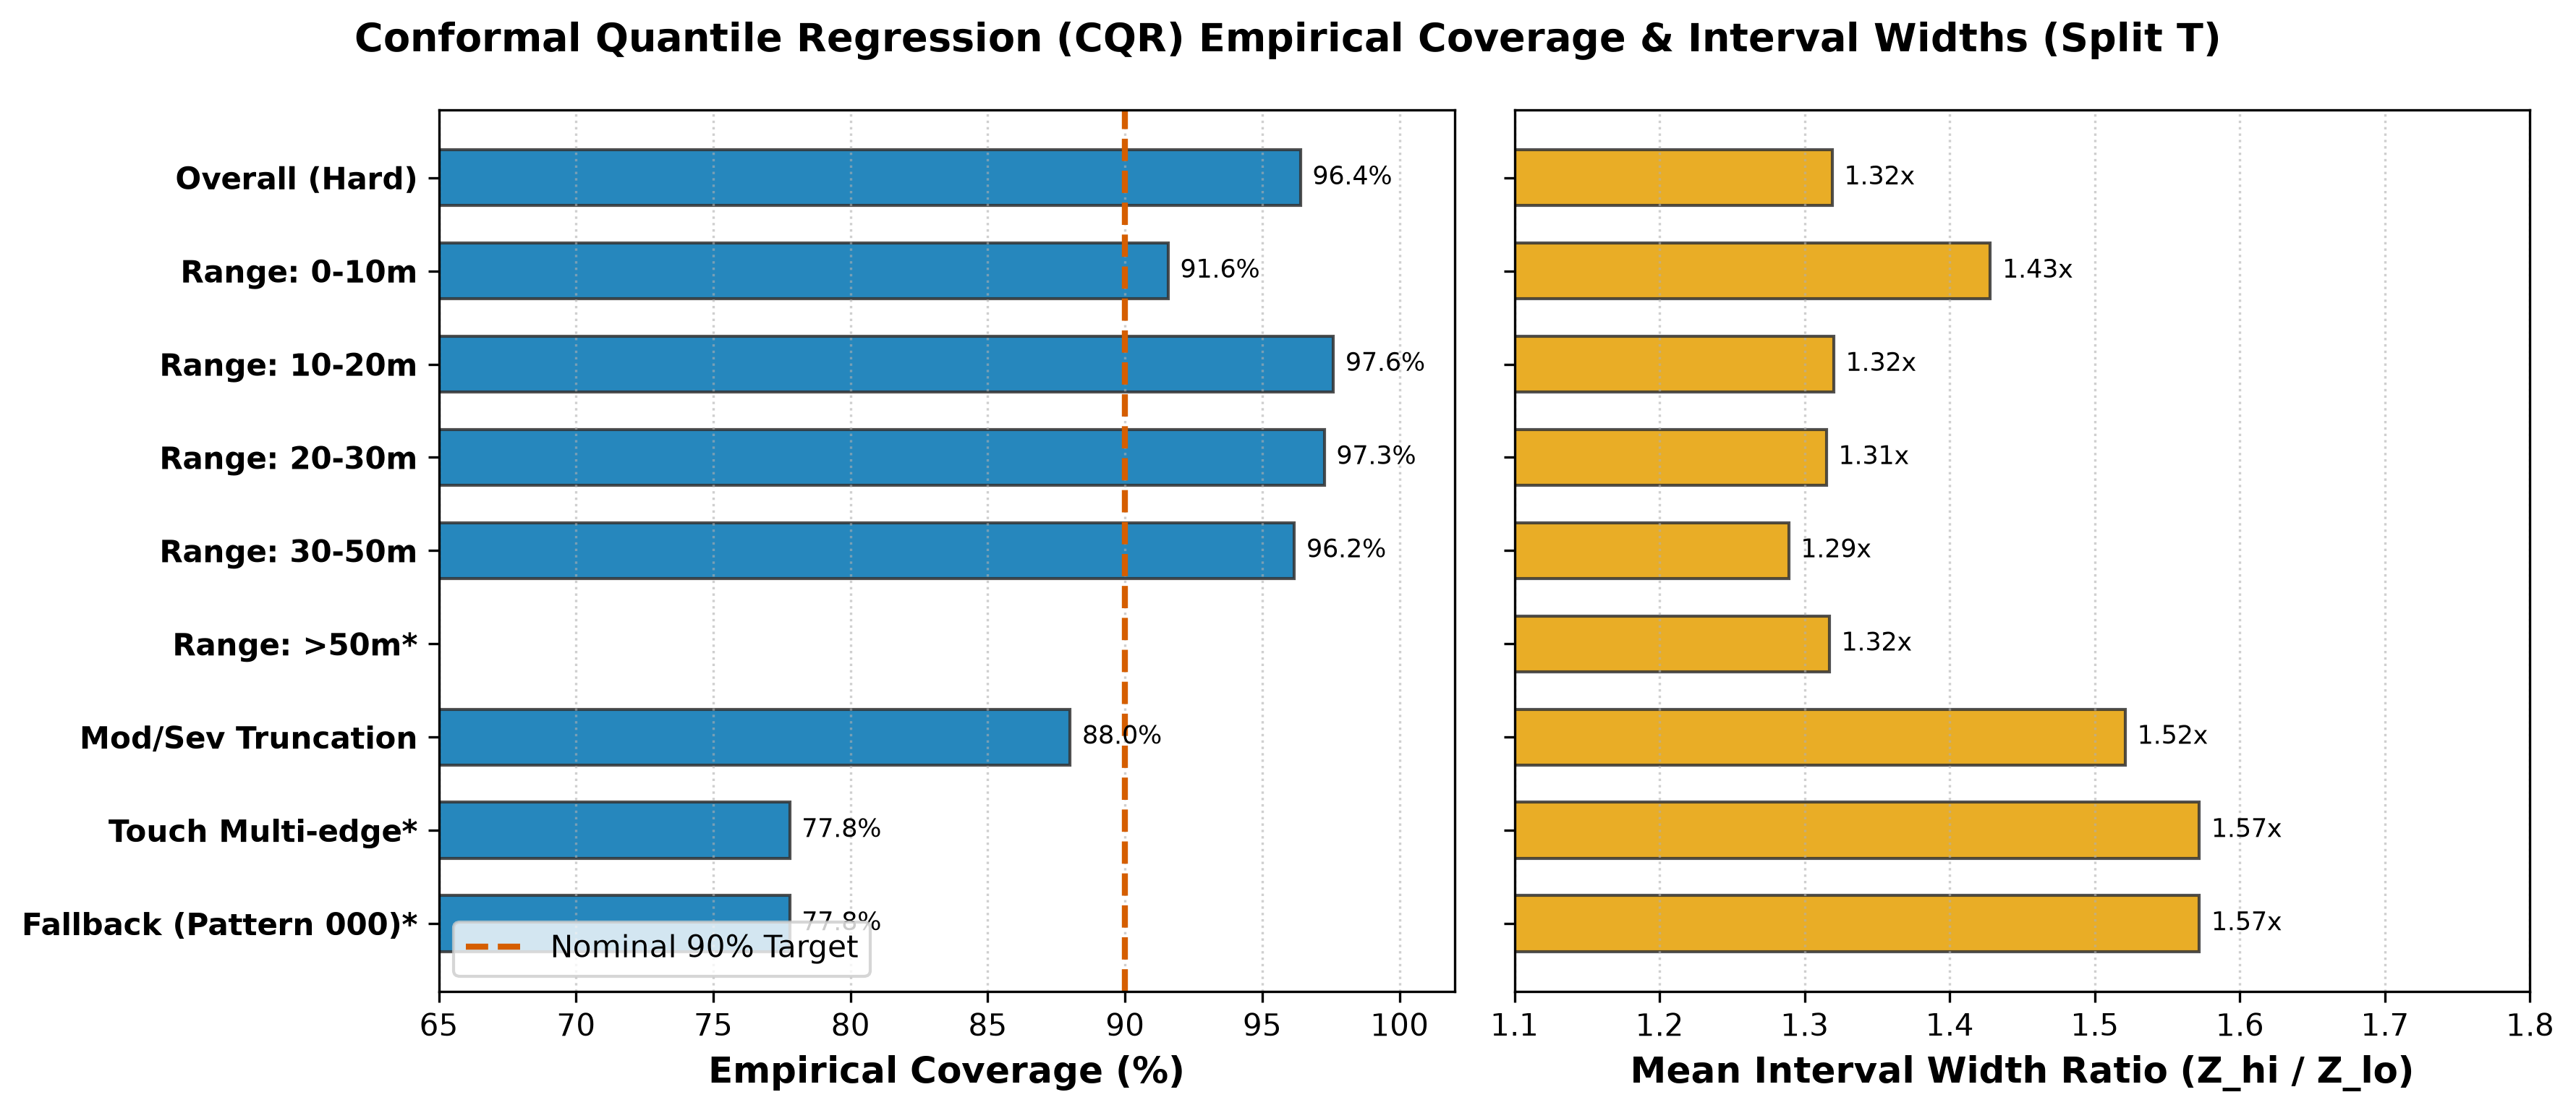
\includegraphics[width=0.98\textwidth]{figures/fig_04_conformal_intervals_and_coverage.png}
\caption{Conformal prediction coverage and interval width trade-offs across ODD domains.}
\label{fig:conformal_intervals}
\end{figure}

\subsection{Hardware Latency Benchmark and Real-Time Viability (RQ4)}
Table~\ref{tab:hardware_latency} reports latency benchmarks measured on 200 in-memory KITTI images:

\begin{table}[htbp]
\centering
\caption{Hardware latency breakdown across GPU and CPU platforms (\texttt{PRELIMINARY-v2}).}
\label{tab:hardware_latency}
\resizebox{\textwidth}{!}{%
\begin{tabular}{llcccccccc}
\toprule
\textbf{Platform \& Execution} & \textbf{Detector} & \textbf{Pre-proc (ms)} & \textbf{Detector FP (ms)} & \textbf{NMS (ms)} & \textbf{Geom (ms)} & \textbf{Resid (ms)} & \textbf{CQR (ms)} & \textbf{Total (ms)} & \textbf{FPS} \\
\midrule
\multirow{3}{*}{\textbf{NVIDIA RTX 5060 Laptop GPU}} & YOLO11s & 9.70 & 26.24 & 0.98 & 0.18 & 0.58 & 0.59 & \textbf{37.99} (P95: 48.49) & \textbf{26.3} \\
\multirow{3}{*}{(FP16 CUDA, static 640$\times$640)} & YOLOv8s & 10.10 & 20.35 & 0.92 & 0.18 & 0.57 & 0.58 & \textbf{32.05} (P95: 57.06) & \textbf{31.2} \\
 & YOLOv5su & 9.80 & 21.42 & 0.88 & 0.18 & 0.60 & 0.60 & \textbf{33.01} (P95: 64.50) & \textbf{30.3} \\
\midrule
\multirow{3}{*}{\textbf{Multi-Core Laptop CPU}} & YOLO11s & 7.60 & 104.32 & 4.31 & 0.22 & 0.62 & 0.64 & \textbf{116.17} (P95: 122.82) & \textbf{8.6} \\
\multirow{3}{*}{(ONNX Runtime FP32, 4 threads)} & YOLOv8s & 7.80 & 131.54 & 4.28 & 0.22 & 0.61 & 0.63 & \textbf{143.37} (P95: 148.60) & \textbf{7.0} \\
 & YOLOv5su & 7.60 & 108.65 & 4.25 & 0.22 & 0.64 & 0.65 & \textbf{120.48} (P95: 124.56) & \textbf{8.3} \\
\bottomrule
\end{tabular}%
}
\vskip 4pt
\parbox{\textwidth}{\footnotesize \textit{Note:} Benchmarks carry the \texttt{PRELIMINARY-v2} label. Pre-processing includes dynamic image resizing, square padding, and host-to-device memory transfer. Post-detector processing accounts for $\approx 1.35\text{ ms}$ ($< 4.2\%$ of total GPU execution time).}
\end{table}

\subsection{Qualitative Error Analysis and Case Studies}
Representative qualitative examples from Split T illustrate the operating characteristics of the hybrid pipeline (shown in Fig.~\ref{fig:case_studies}):
\begin{itemize}
    \item \textbf{Oblique Viewing Angles:} For lateral vehicles (e.g., frame \texttt{000006}, $Z_{\text{gt}} = 19.72\text{ m}$), width cue $Z_w$ underestimates distance significantly ($Z_w = 9.81\text{ m}$) due to vehicle length projection. The residual model corrects this distortion, producing $\hat{Z}_f = 20.60\text{ m}$ ($4.48\%$ error) and a valid conformal interval of $[17.44, 23.63]\text{ m}$.
    \item \textbf{Near-Field 3D Center Offset:} At close range (frame \texttt{000385}, $Z_{\text{gt}} = 7.91\text{ m}$), pure geometry measures distance to the nearest vehicle surface, underestimating center distance ($Z_d = 7.02\text{ m}$, $-11.2\%$). The residual model compensates for vehicle half-length offset, yielding $\hat{Z}_f = 7.99\text{ m}$ ($0.96\%$ error).
    \item \textbf{Severe Image Boundary Clipping:} When vehicles touch image borders (frame \texttt{000152}, truncation 0.35, representing 1.3\% of True Positives), perspective cues are clipped. The direct regression fallback and widened CQR interval ($[4.08, 7.07]\text{ m}$) safely cover the true distance ($Z_{\text{gt}} = 6.37\text{ m}$).
    \item \textbf{Failure Cases:} Out-of-interval predictions occur predominantly on severely cropped corner objects undergoing complex aspect distortion (frame \texttt{001414}, $Z_{\text{gt}} = 5.92\text{ m}$, $\hat{Z}_f = 8.46\text{ m}$, Interval $[7.05, 10.52]\text{ m}$).
\end{itemize}

\begin{figure}[htbp]
\centering
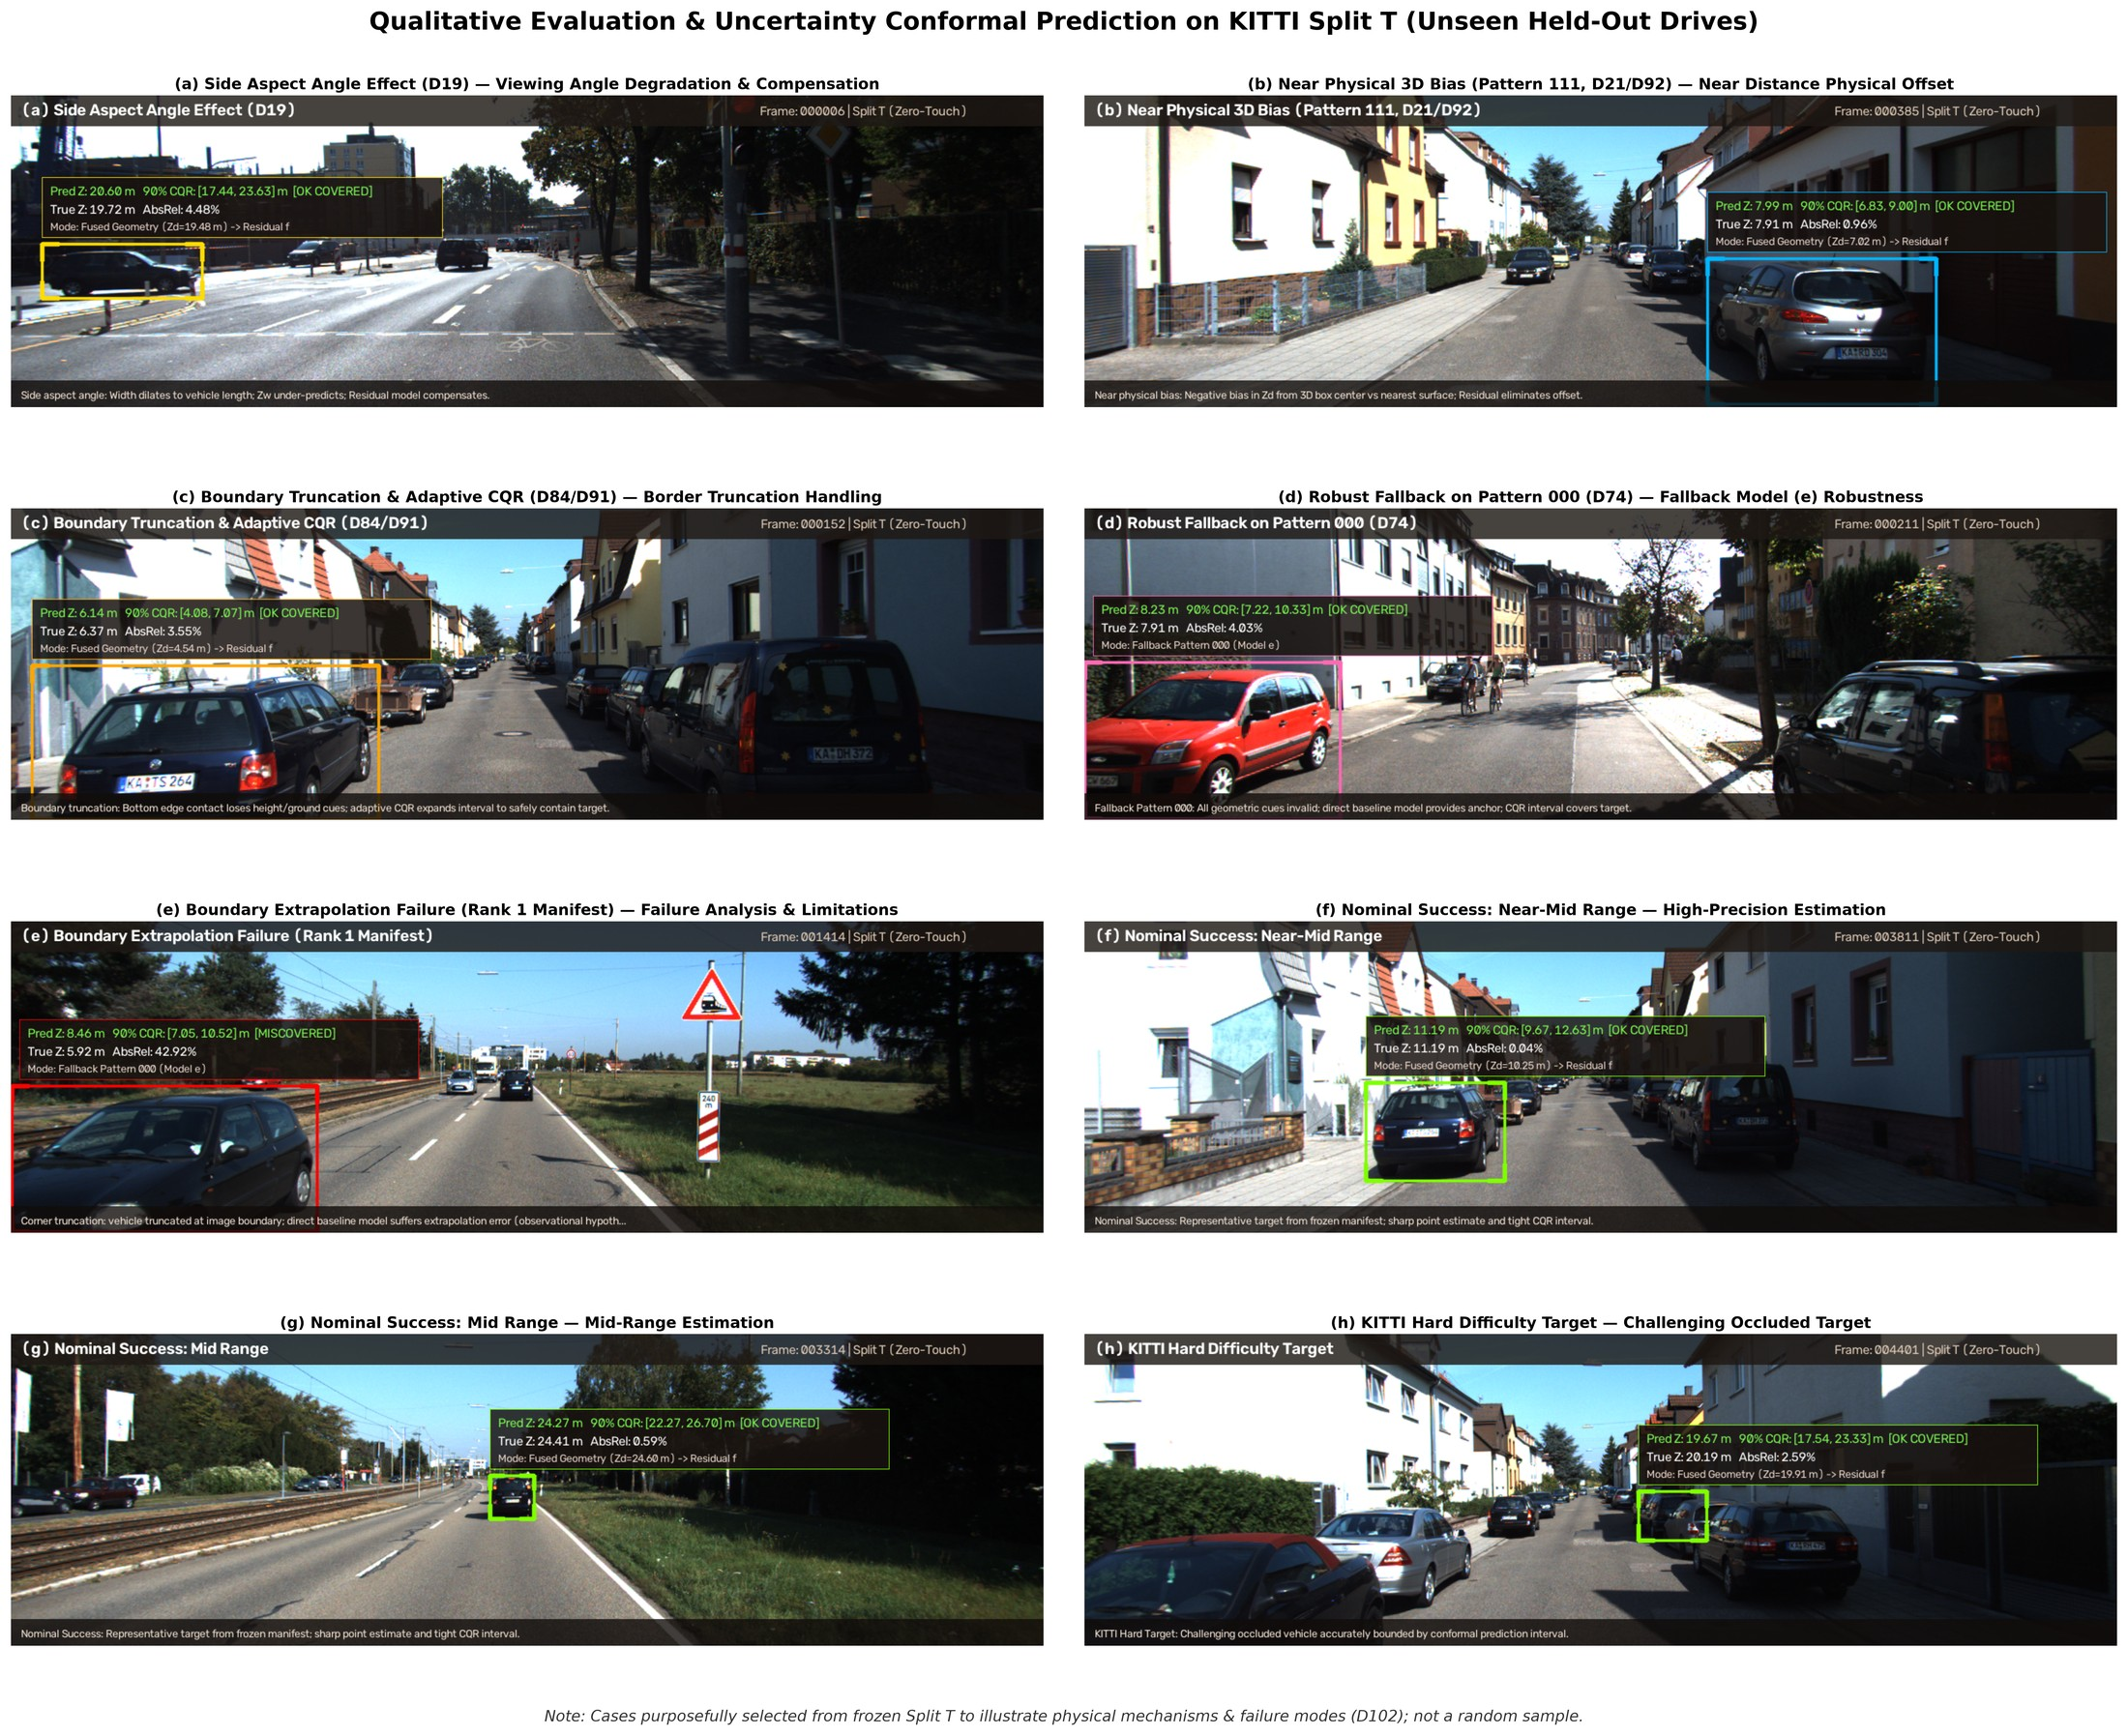
\includegraphics[width=0.98\textwidth]{figures/fig_05_qualitative_case_studies.jpg}
\caption{Representative qualitative case studies on held-out test Split T.}
\label{fig:case_studies}
\end{figure}

% -------------------------------------------------------------------------
% 6. LIMITATIONS AND THREATS TO VALIDITY
% -------------------------------------------------------------------------
\section{LIMITATIONS AND THREATS TO VALIDITY}
\label{sec:limitations}

We explicitly document 14 methodological and practical limitations governing our study:
\begin{enumerate}
    \item \textbf{Truck Class Distribution Imbalance \& Single-Dataset Domain Constraint:} Heavy vehicles (Trucks) are concentrated in specific sequences ($4.8\%$ in Split A vs $1.3\%$ in Split T), precluding robust cross-class generalization. Furthermore, evaluation is confined to daytime, clear-weather KITTI scenes; adverse conditions (rain, fog, night) remain unvalidated.
    \item \textbf{Survivorship Bias on True Positives and Target Matching Scope:} All ranging evaluations are conditioned on True Positive detections (recall $82.8\%\text{--}84.4\%$). Detection mAP@0.7 is intentionally not evaluated. Operational risk in open-world driving includes false negative misses ($26.2\%\text{--}29.3\%$ at 30--50 m, and $72.7\%\text{--}93.9\%$ beyond 50 m on Split T).
    \item \textbf{Sparse Distant Sample Support (>50 m):} Ground Truth Car Hard objects beyond 50 m comprise only 33 instances on Split T, yielding $\le 9$ True Positives. Ranging metrics in this regime must be regarded as exploratory.
    \item \textbf{Drive Concentration and Cluster Correlation:} Evaluation clusters are small ($k = 10$ drives in Split T, $k = 12$ in Split B), below the recommended threshold of $k \ge 20$ for asymptotic cluster bootstrap validity.
    \item \textbf{Detector Training Checkpoint Reproducibility and Single-Seed Training:} All detectors were optimized under a single random seed (seed 42), precluding multi-seed detector variance estimation.
    \item \textbf{KITTI Neighbor Class Matching Protocols and Restricted Training Scale:} Unlike the official KITTI evaluation server, neighboring classes (Van, Truck) are not ignored, slightly depressing precision. Detectors were trained on $\approx 50\%$ of available KITTI data (Split A) to preserve drive disjointness.
    \item \textbf{Indirect Qualitative Design Leakage and Flat Ground-Plane Assumption:} Boundary masking heuristics were informed by preliminary explorations before split freezing. Ground cue $Z_g$ relies on a planar road assumption vulnerable to slopes and vehicle pitch.
    \item \textbf{Empirical Indistinguishability of Residual and Direct Regression \& Vehicle Viewing Angle:} Residual Model (f) and Direct Model (e) exhibit overlapping confidence intervals on Split T. Fixed calibrated priors assume frontal/rear orientation; oblique angles distort bounding box cues.
    \item \textbf{Post-Hoc Verification Transparency:} The initial Split T run experienced inflated errors due to an XGBoost \texttt{base\_score} string serialization formatting bug. This was resolved post-hoc via JSON scalar standardization without model retraining or hyperparameter modification.
    \item \textbf{Exchangeability Shift and Conservative Over-Coverage:} Domain difficulty differences between Split C and Split T violate strict exchangeability, resulting in conservative over-coverage ($96.39\%$).
    \item \textbf{Optimism of 10-Cluster Bootstrap CIs:} Intra-split bootstrap intervals underestimate total cross-split partition sensitivity ($\sigma \approx 7\%\text{--}9\%$).
    \item \textbf{Masked Local Under-Coverage:} Pooled 96\% coverage conceals local vulnerabilities: truncated vehicles ($88.0\%$) and boundary fallback cases ($77.8\%$) remain below nominal 90\% coverage.
    \item \textbf{Mondrian Interval Width Inflation:} Mondrian grouping restores coverage in near distance regimes ($94.1\%$) but inflates interval width by $1.43\text{--}1.47\times$.
    \item \textbf{Hardware and Latency Benchmark Constraints:} GPU benchmarks utilize static $640 \times 640$ square padding rather than dynamic letterboxing, increasing pixel processing overhead by $\approx 2.9\times$. Latency figures carry the preliminary benchmark label.
\end{enumerate}

% -------------------------------------------------------------------------
% 7. CONCLUSION AND FUTURE WORK
% -------------------------------------------------------------------------
\section{CONCLUSION AND FUTURE WORK}
\label{sec:conclusion}

We presented a calibrated hybrid monocular distance estimation framework integrating perspective geometry with gradient-boosted residual calibration and conformalized quantile regression for lightweight YOLO detectors. By establishing a strict drive-disjoint evaluation protocol (\texttt{splits-v2}) on the KITTI benchmark, we demonstrated that:
\begin{enumerate}
    \item Perspective geometry provides a physically grounded baseline, isolating vehicle height as the dominant physical anchor;
    \item Bounding box pixel jitter in mature lightweight detectors has near-zero monotonic correlation with ranging error;
    \item While learned residual correction achieves numerical precision comparable to direct regression on Split T, it confers substantial data efficiency ($68\%$ error reduction under data scarcity) and bounds extrapolation errors beyond 30 meters;
    \item Conformal prediction intervals provide actionable safety bounds, though sequence-level cluster heterogeneity significantly impacts empirical coverage stability across alternate drive partitions.
\end{enumerate}

Future investigations will explore multi-camera temporal tracking (Kalman filtering), embedded INT8 quantization on automotive edge hardware, and domain adaptation across adverse weather conditions.

% -------------------------------------------------------------------------
% DECLARATIONS AND SCIENTIFIC INTEGRITY
% -------------------------------------------------------------------------
\section*{DECLARATIONS AND SCIENTIFIC INTEGRITY}
\begin{itemize}
    \item \textbf{Originality \& Anti-Plagiarism:} This paper reports original experimental results. All figures, tables, and numerical metrics are directly derived from reproducible, version-controlled benchmark artifacts.
    \item \textbf{AI Tool Usage Disclosure:} Generative AI tools were employed exclusively for editorial polishing, code structuring, and formatting assistance. All scientific claims, experimental protocols, model training, and data interpretations were authored and verified by the research team.
    \item \textbf{Reproducibility:} Code, configurations, split definitions, and evaluation scripts are structured for complete reproducibility.
\end{itemize}

% -------------------------------------------------------------------------
% REFERENCES
% -------------------------------------------------------------------------
\bibliographystyle{spiebib}
\bibliography{references}

\end{document}
